%%____________________________________________________________________________||
\section{Systematic uncertainties in the \mht dimension}
\label{sec:mhtTemplate}

The estimate of the number of events per (\njet,\nb,\scalht) bin,
integrated over \mht, is determined from data control samples, with
the associated systematic error determined from closure tests
described in Section \ref{sec:syst-from-closure}. This section
describes the method used to determine the systematic uncertainties in
the distribution of events according to \mht. A data driven approach is
utilised where the level of closure in the control regions is used
to determine the maximum deviation expected in the signal region.

When looking at the \mht dimension inclusively there are
large theoretical uncertainties that originate from mixing events
at different scales. However, if a a variable, such as \scalht, 
that is strongly correlated with the scale of the event 
is used to 'set the scale' these uncertainties can be mitigated.
In \ref{sec:valid8} the 8 TeV data will be used to show that binning in
\scalht elminates bias in the data and MC agreement in the control regions. 
In \label{sec:systMhtDimension} this will then be used to extract systematic template 
variations in the signal region. In \ref{sec:syst13TeV} results for the
expected systematic for Run 2 will be shown. Finally, in \ref{sec:addMhtUnc} 
methods for dealing with additional template uncertainties are discussed.


% extent to which the control regions can constrain this bias 
% to the flat hypothesis
%Motivated by the inclusive distribution, a linear bias is assumed.

\subsection{Validation with 8 \TeV Data}
\label{sec:valid8}
In previous versions of this analysis three control regions
were used: \mj, \mmj and \gj. In Figure~\ref{fig:linearMotiv} the data/MC 
distribution against \mht for the control region selection 
(detailed in \cite{CMS_AN_2013-366}) is shown inclusive 
in \scalht and categories. By fitting a second order orthogonal polynomial
it can be seen that in each case the quadratic term is small and consistent
with zero. Motivated by this a linear function will be used to measure
the level of bias remaining when the \mht dimension is binned in \mht. 
As the normalisation systematic is dealt with seperately the normalisation
of the MC is set to that of the data when fitting alternative templates.

\begin{figure}[h!]
  \centering
  \subfigure[\gj]{
    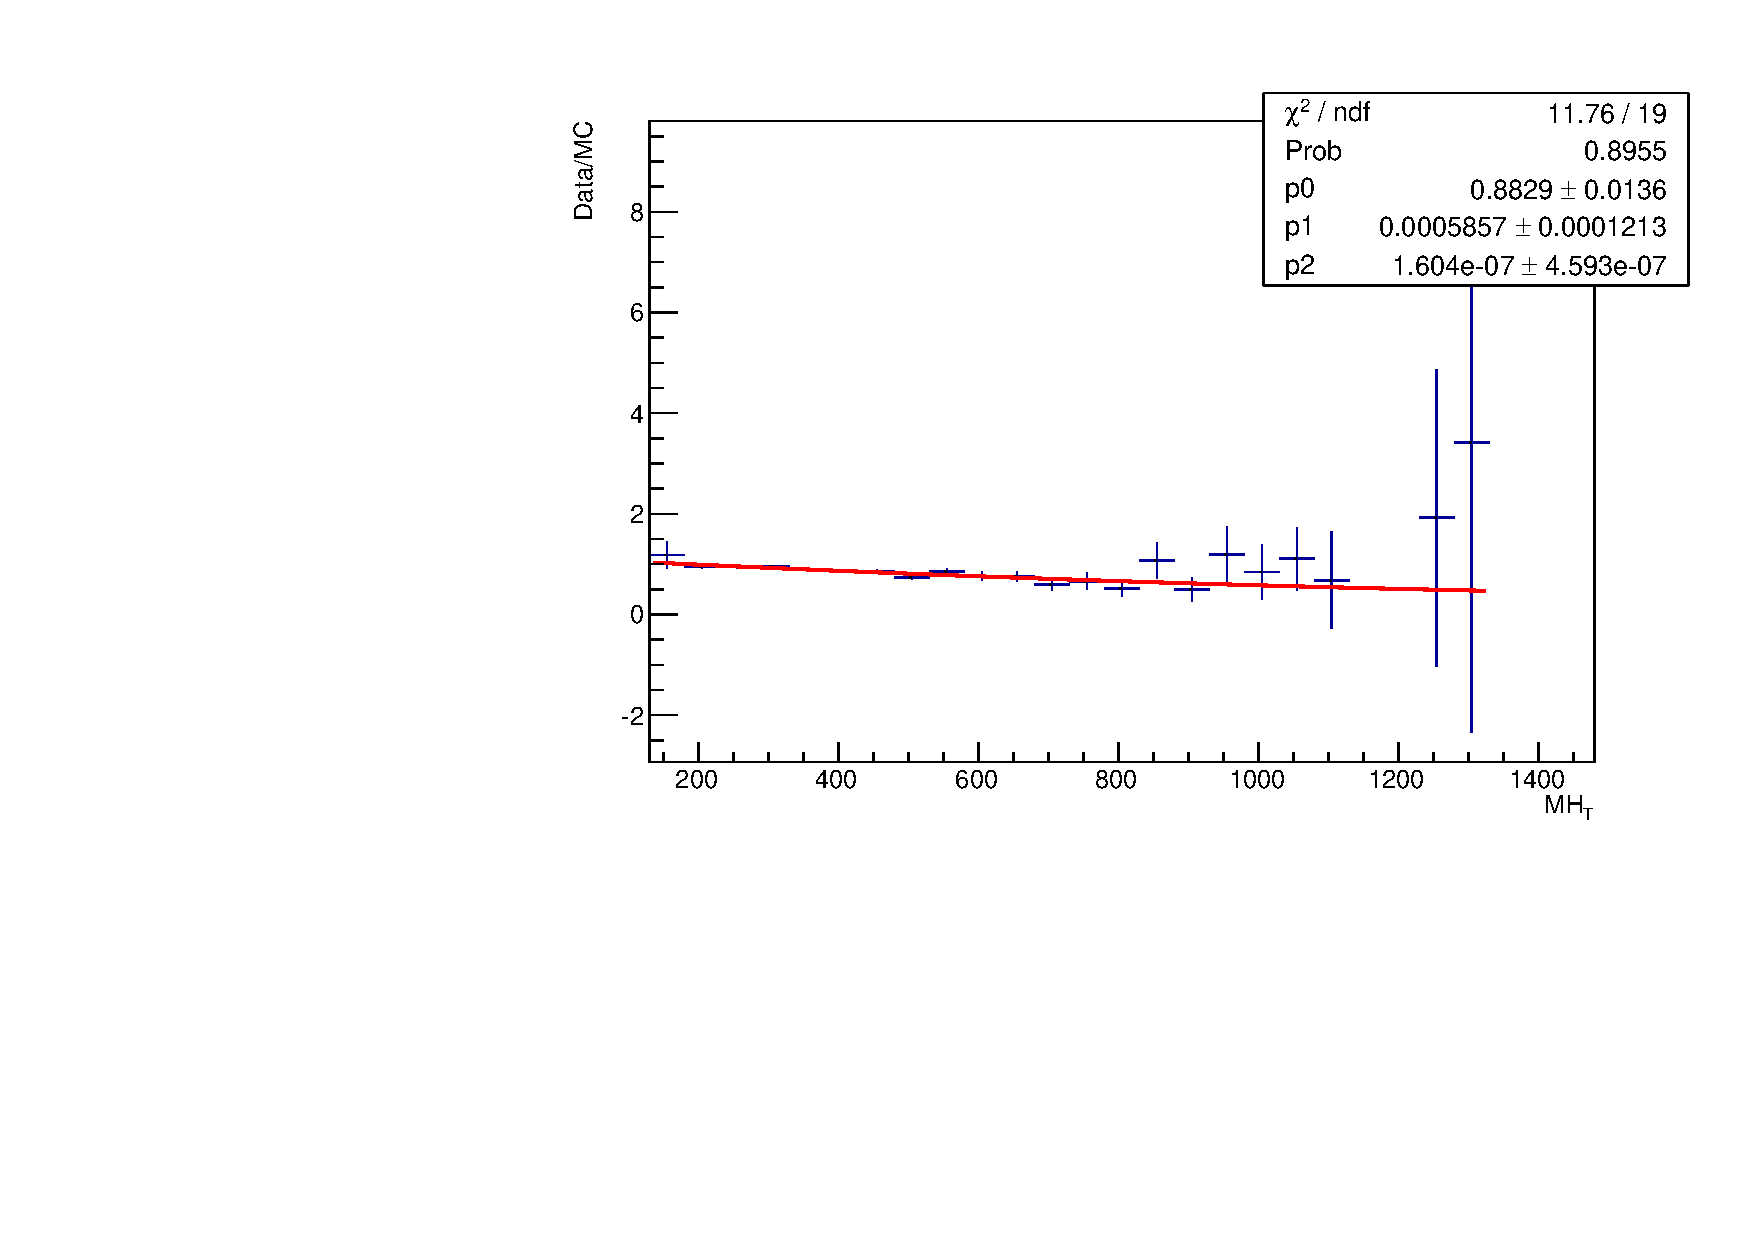
\includegraphics[width=0.5\textwidth]{figures/template/quadratic/mht_Inc_Inc_ht_Inc_SinglePhoton_Quadratic.pdf}
  }~~
  \subfigure[\mmj]{
    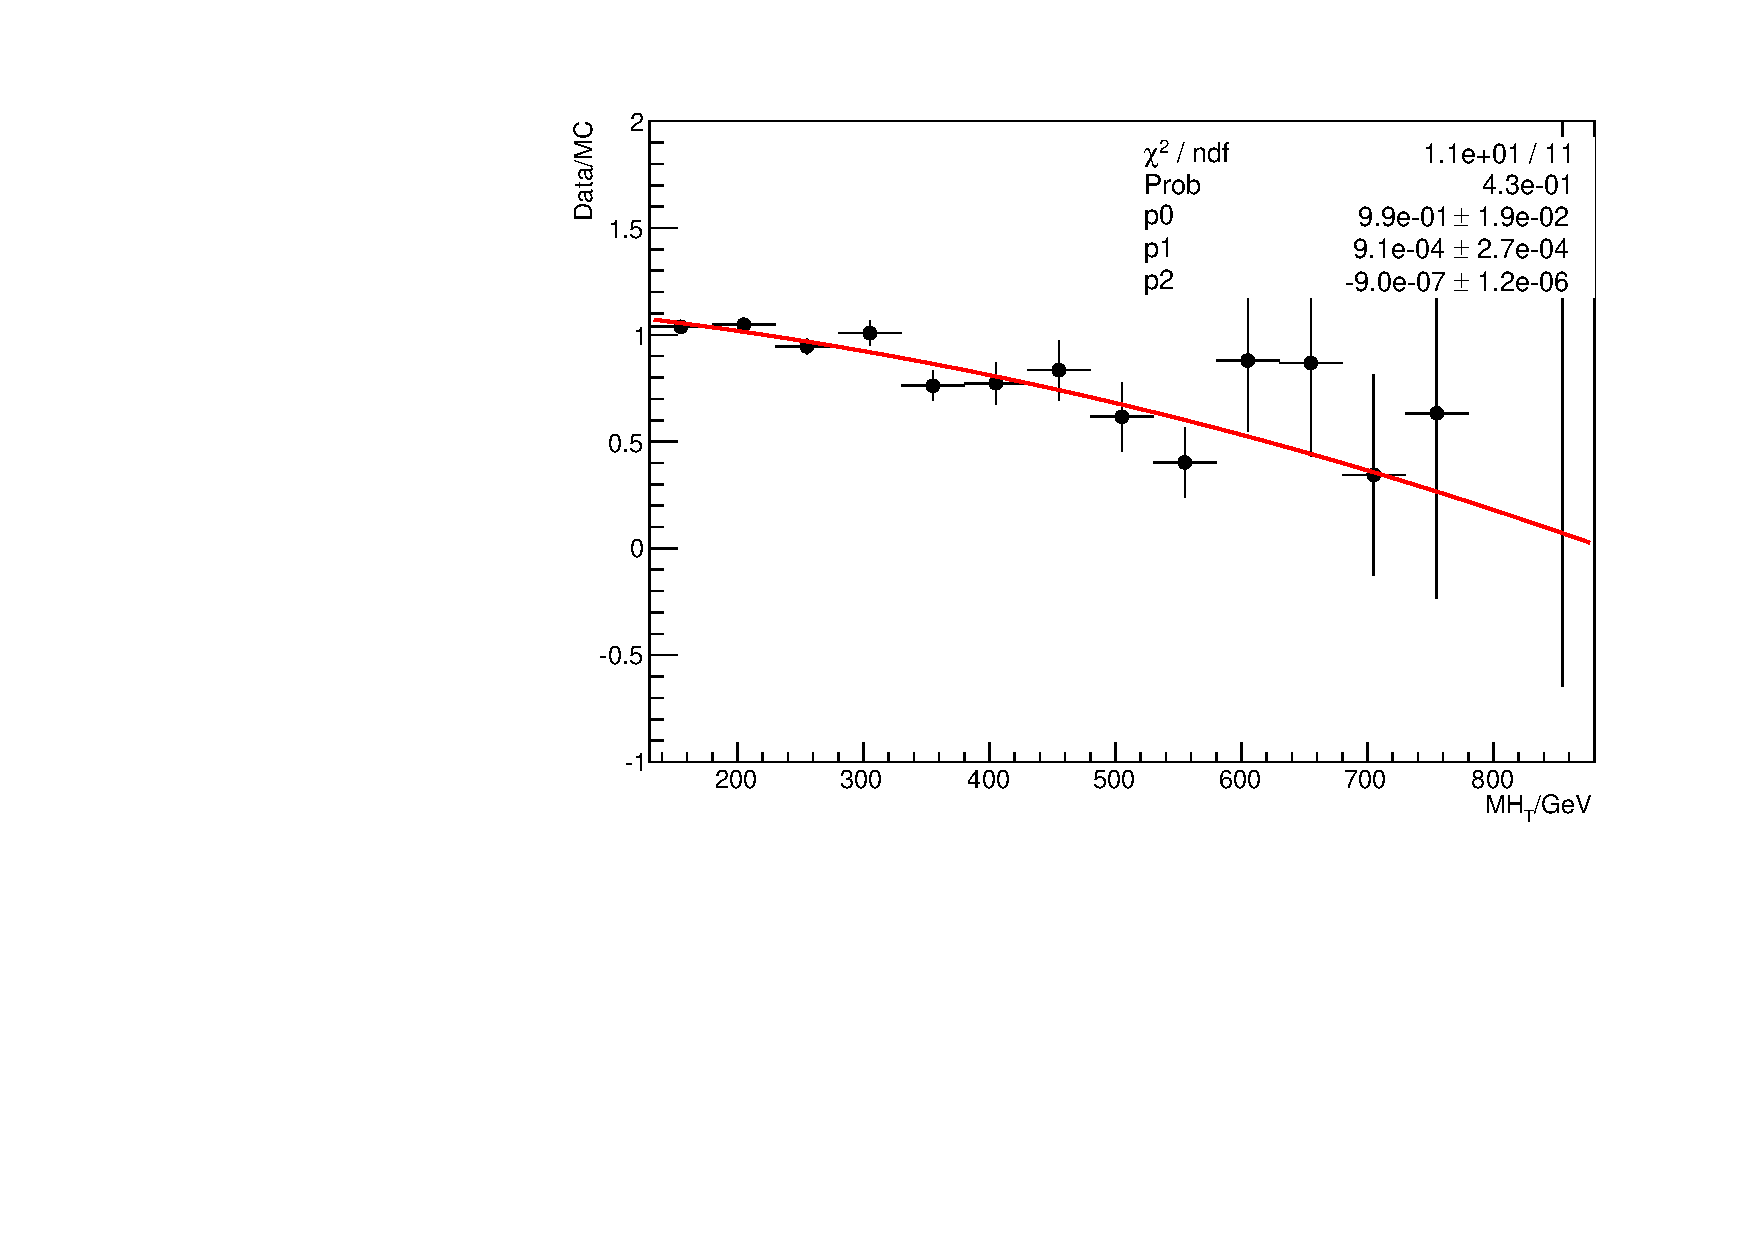
\includegraphics[width=0.5\textwidth]{figures/template/quadratic/mht_Inc_Inc_ht_Inc_DoubleMu_Quadratic.pdf}
  }\\
  \subfigure[\mj]{
    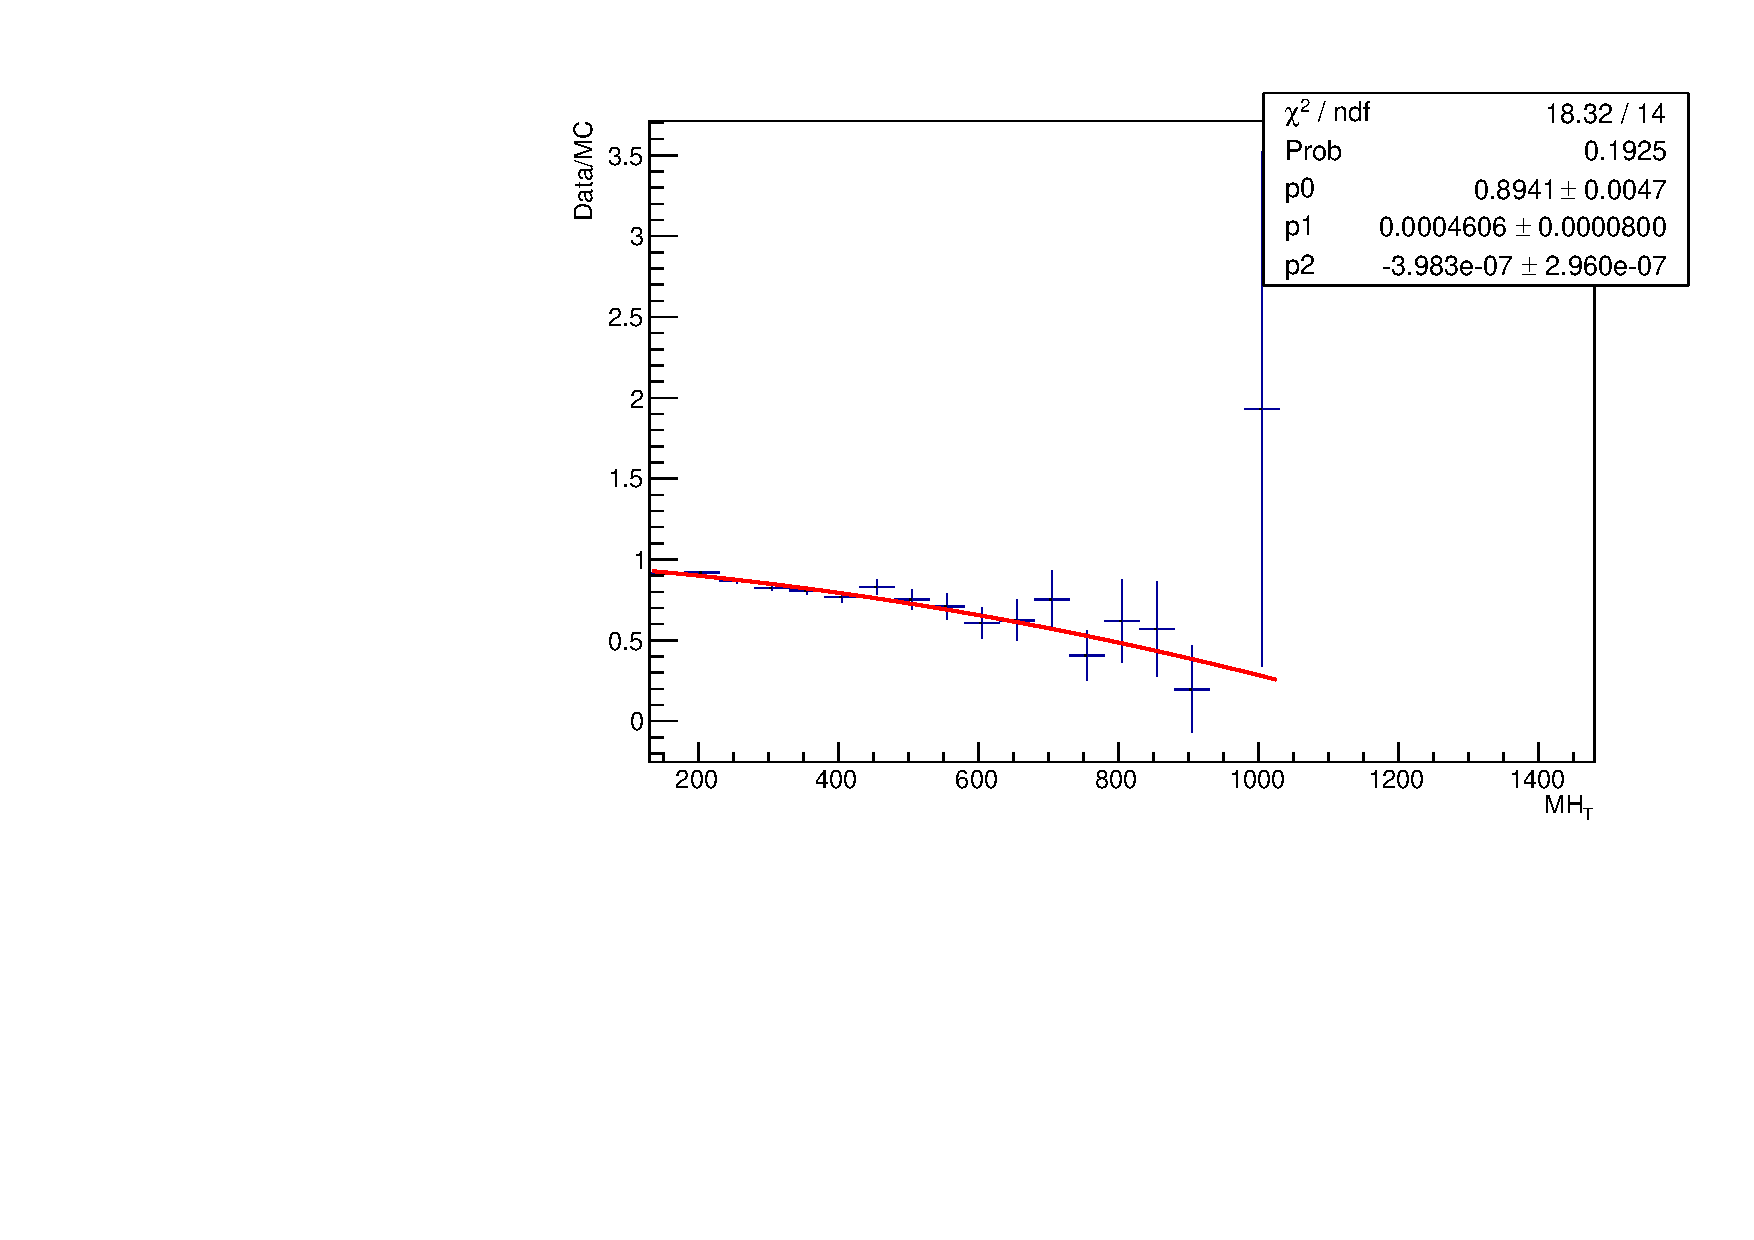
\includegraphics[width=0.5\textwidth]{figures/template/quadratic/mht_Inc_Inc_ht_Inc_SingleMu_Quadratic.pdf}
  }~~
  \\
  \caption{\label{fig:linearMotiv} 
  The data/MC distribution against \mht for an inclusive selection on category and \scalht
  showing the results of a quadratic fit. There is a clear bias
  in the linear component while the quadratic component is consistent with zero.
}
\end{figure}

By anchoring the scale using binning in the \scalht dimension the remaining
bias should be negligible. In Figures~\ref{fig:linearFits0bLe3} and \ref{fig:linearFits0bGe4} 
example fits of an orthogonal linear function to the data/MC ratio 
are shown for the three control regions. Comparing to the inclusive distribution 
the linear component can be seen to be much more compatible with the null, 
zero bias hypothesis. In order to formalise this assertion 
the pull of the linear component from zero is calculated.
This pull distribtuion is shown for each of the three control regions in
in Figure~\ref{fig:pulls} and can be see in each case to have mean and sigma
consistent with zero and one respectively. This supports the zero
bias hypothesis. Figure~\ref{fig:frenchFlagPulls} shows the distribution of the pulls 
in category and \scalht bins. Those anchored by \scalht are consistent
with zero (including inclusive categories) while fits inclusive in \scalht
show very large pulls. This shows as expected the \scalht anchoring
is critical for removing bias in the \mht dimension.  

\begin{figure}[h!]
  \centering
  \subfigure[\gj]{
    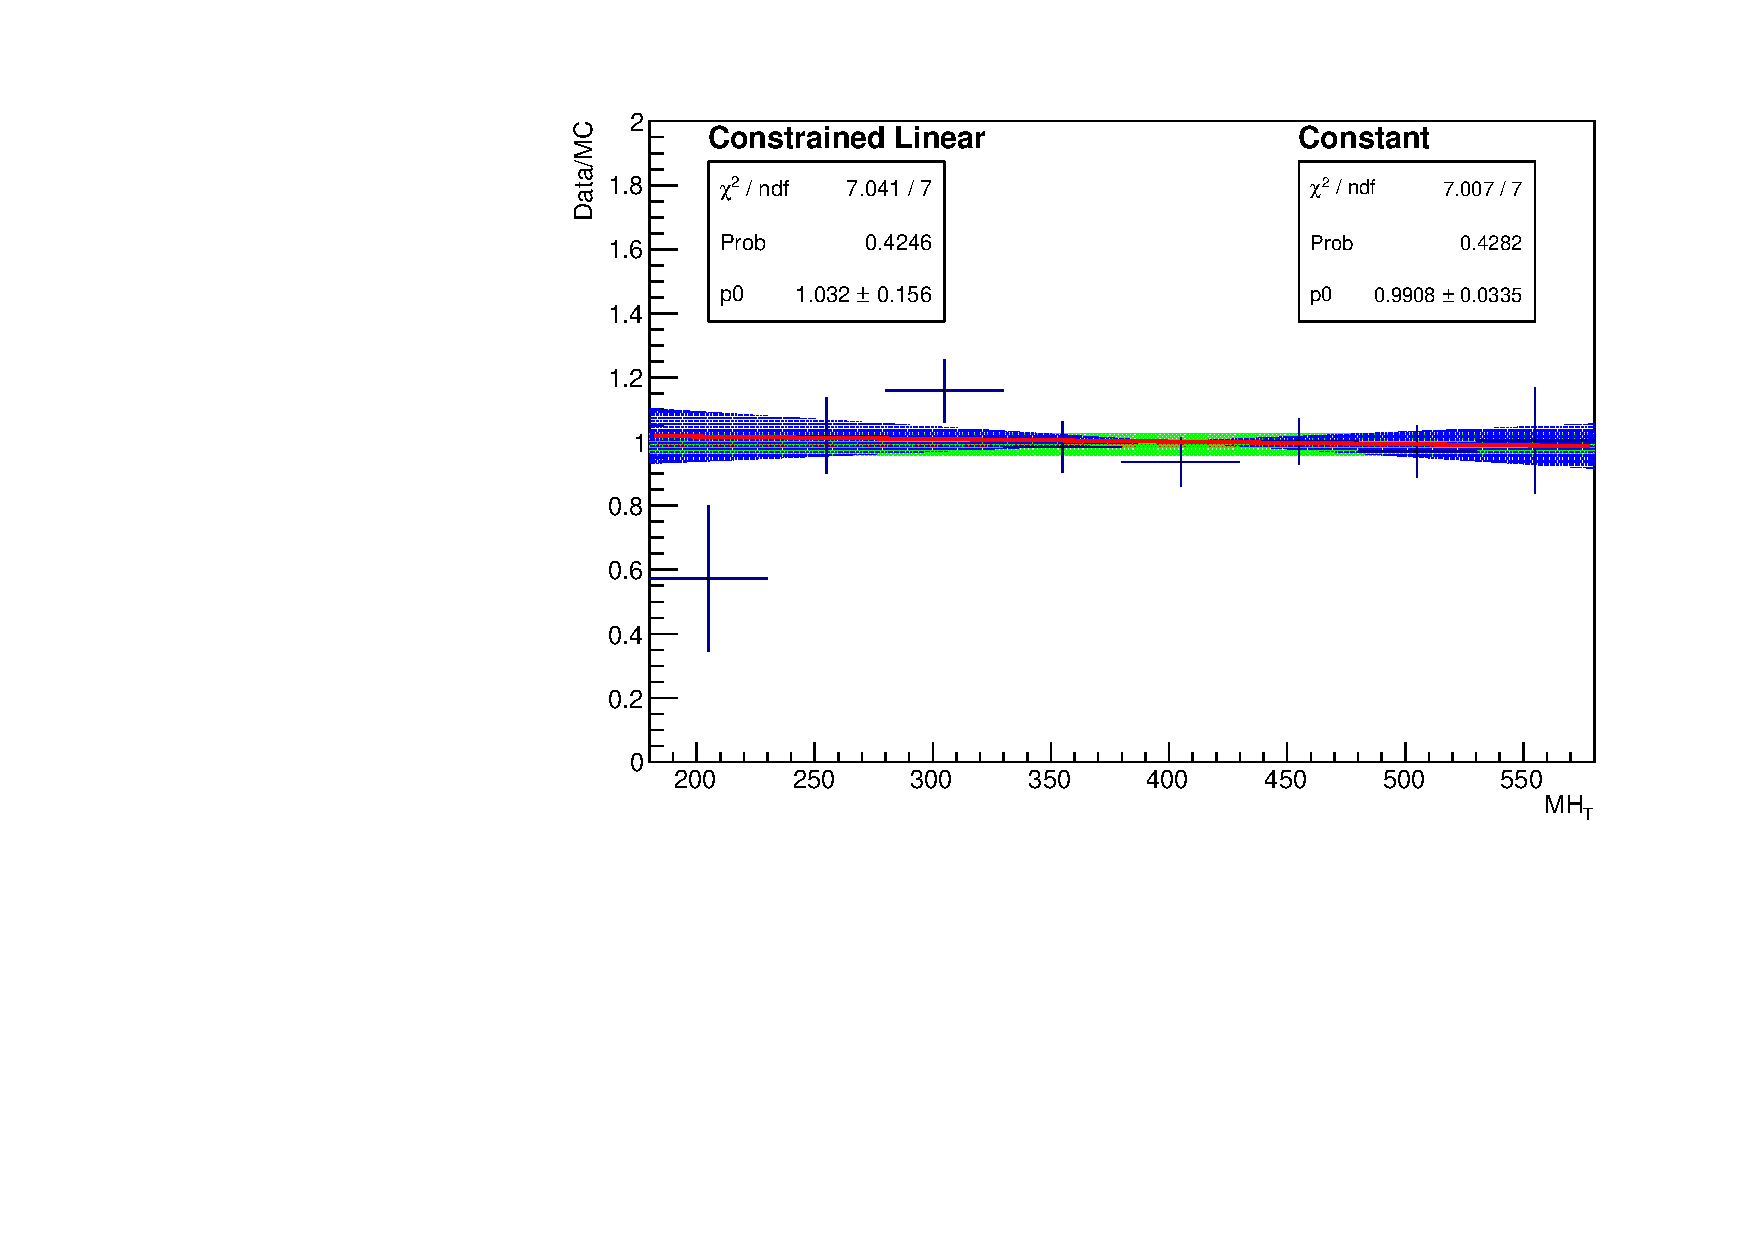
\includegraphics[width=0.5\textwidth]{figures/template/linear/mht_eq0b_le3j_ht_475_575_SinglePhoton.pdf}
  }~~
  \subfigure[\mmj]{
    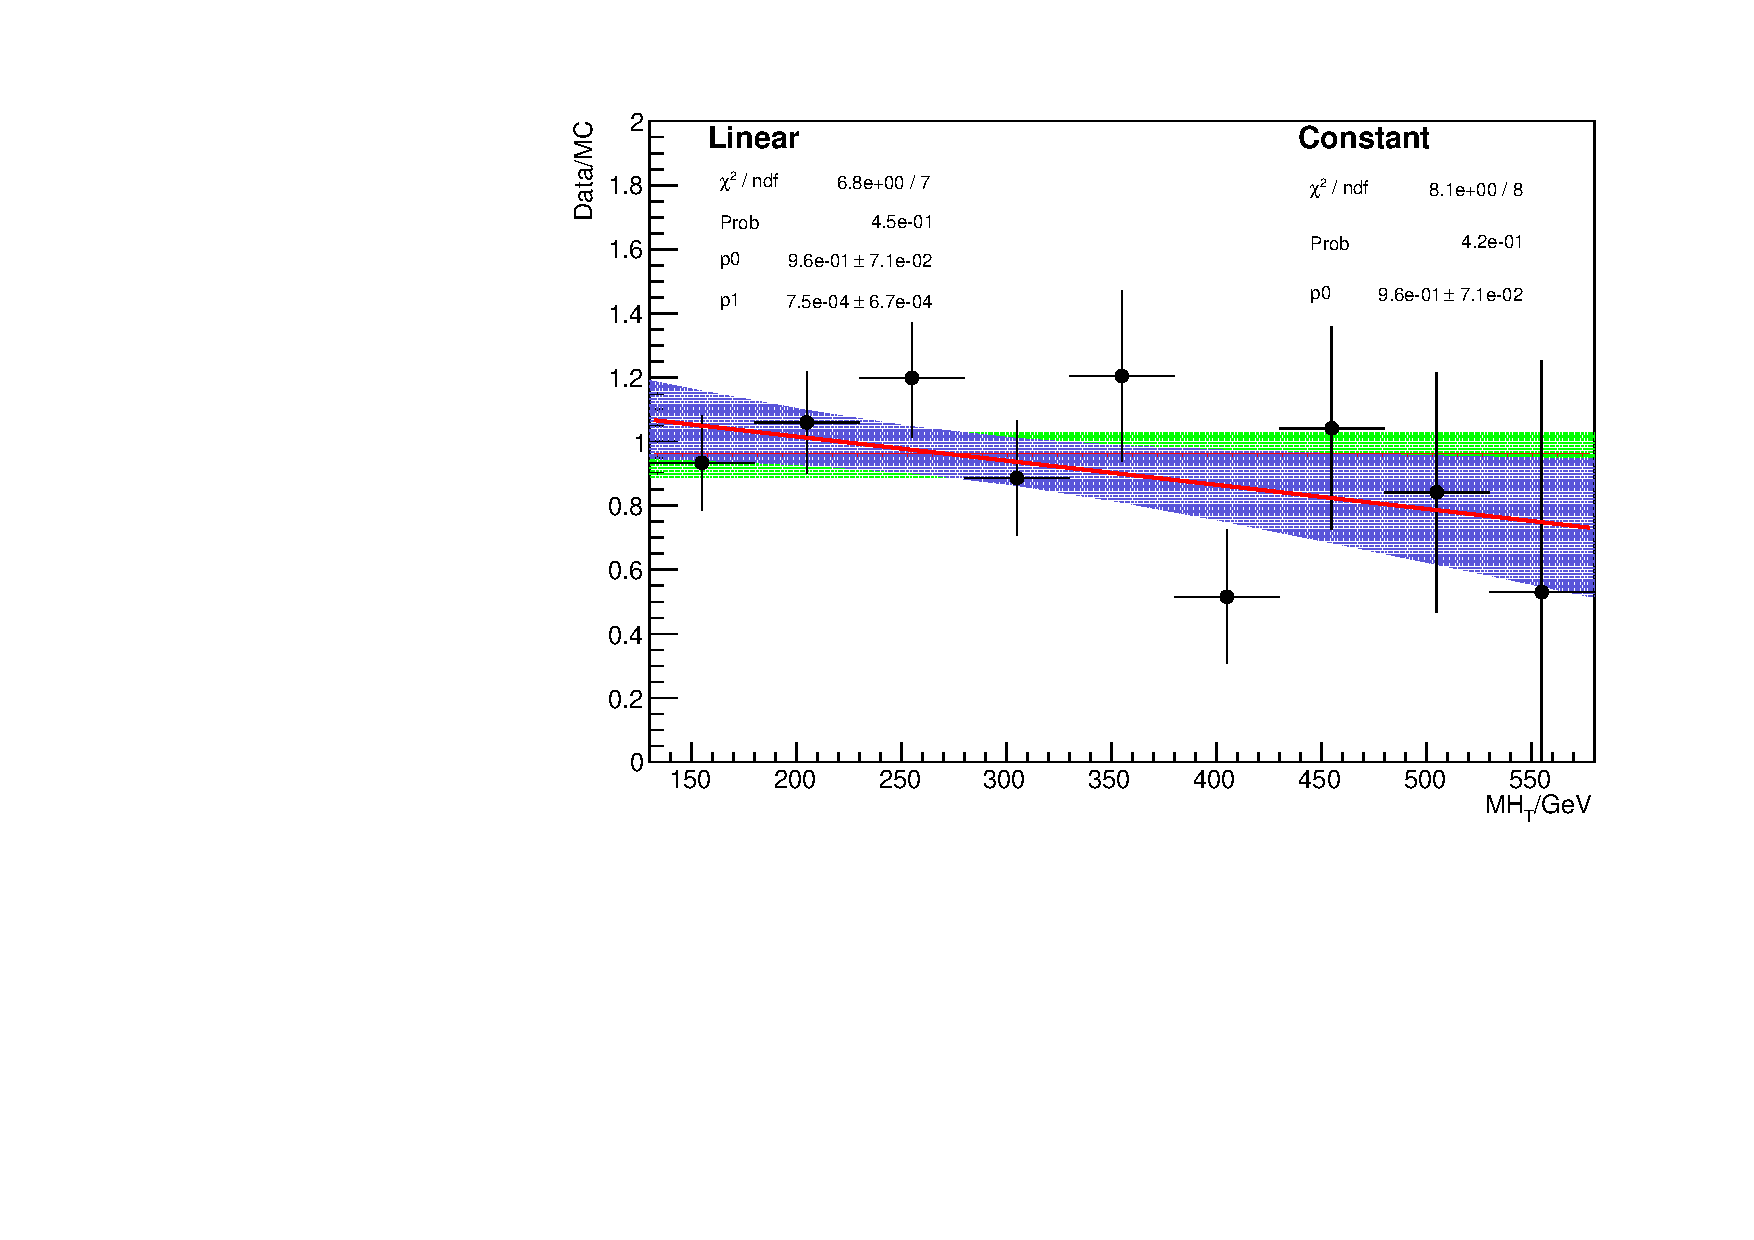
\includegraphics[width=0.5\textwidth]{figures/template/linear/mht_eq0b_le3j_ht_475_575_DoubleMu.pdf}
  }\\
  \subfigure[\mj]{
    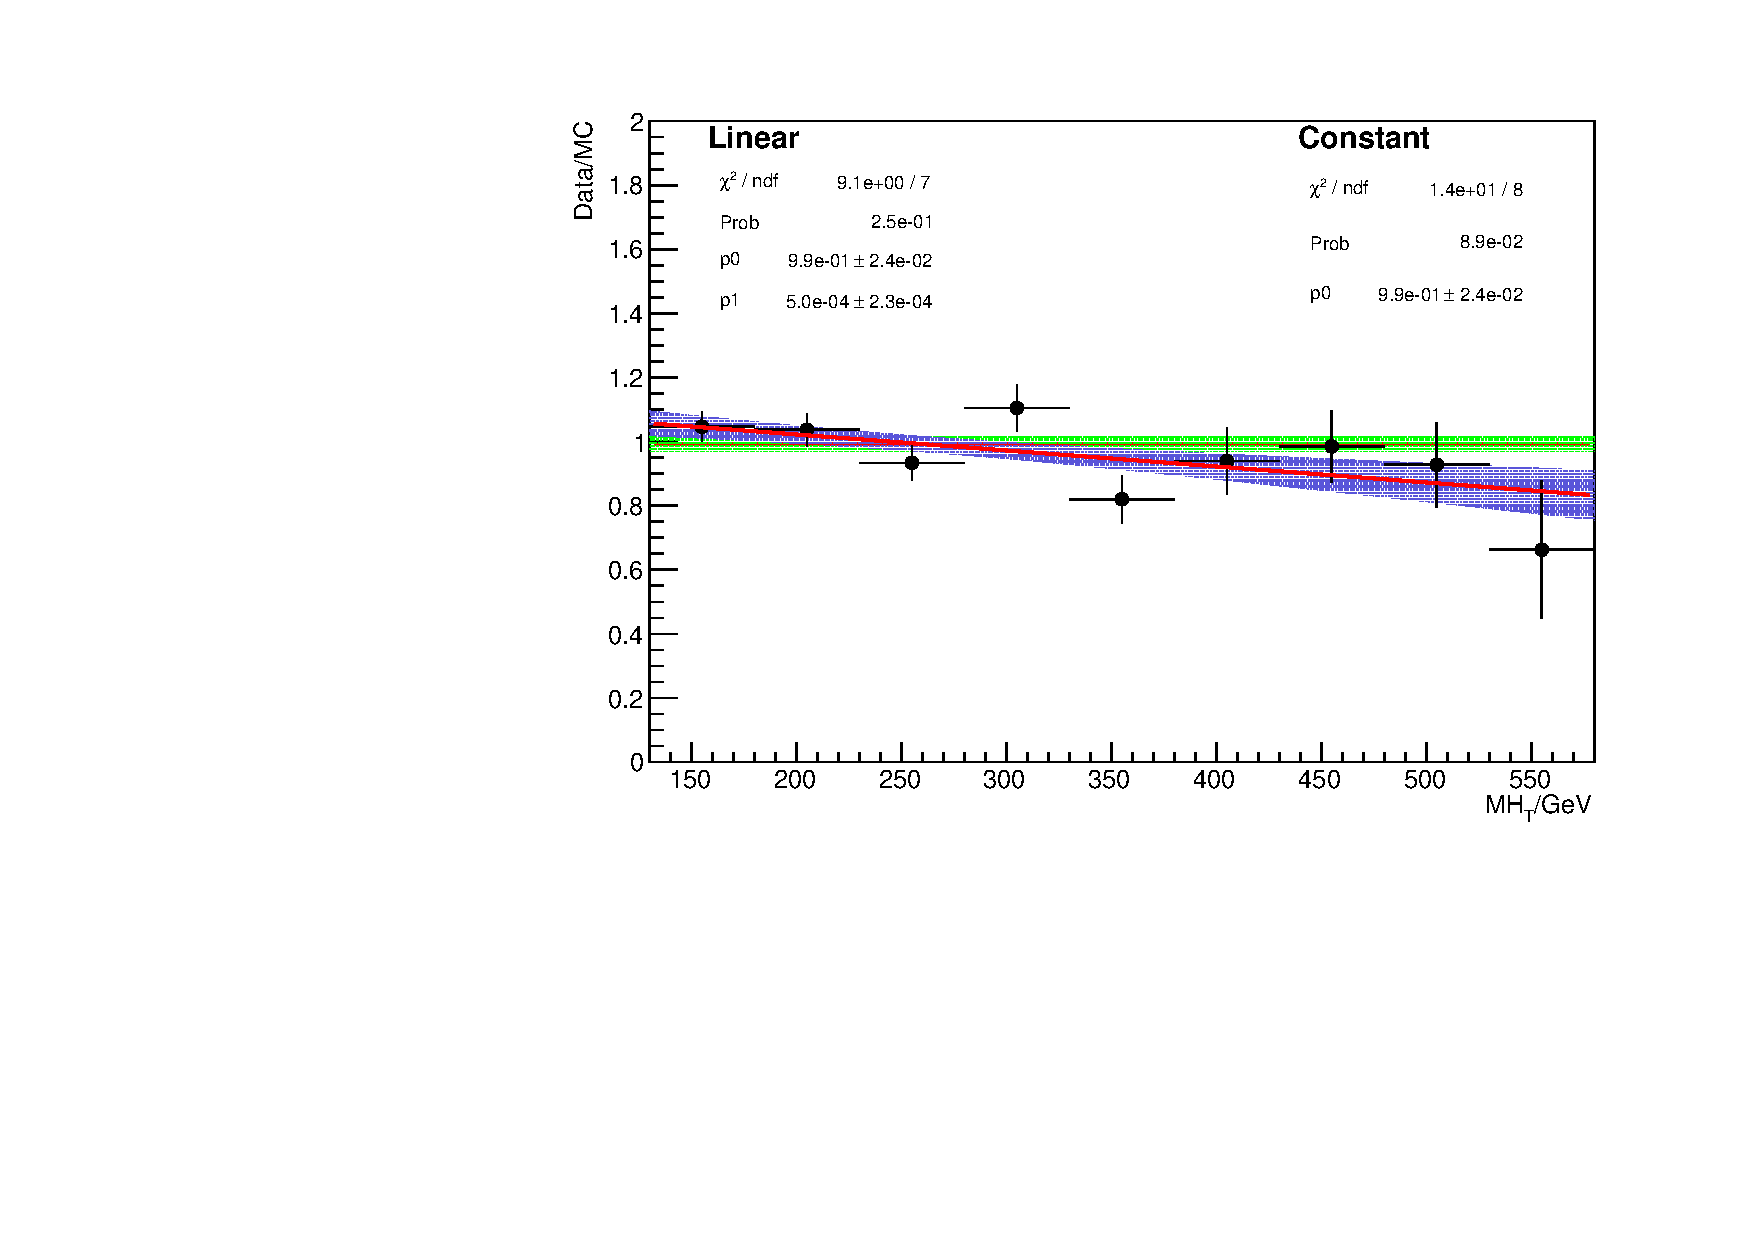
\includegraphics[width=0.5\textwidth]{figures/template/linear/mht_eq0b_le3j_ht_475_575_SingleMu.pdf}
  }~~
  \\
  \caption{\label{fig:linearFits0bLe3} 
  The data/MC distribution against \mht for the 0b, $\le3$j category and \scalht 475-575\GeV bin.
  The large linear bias in the linear component seen in Figure~\ref{fig:linearMotiv} is
  largely mitigated.
}
\end{figure}

\begin{figure}[h!]
  \centering
  \subfigure[\gj]{
    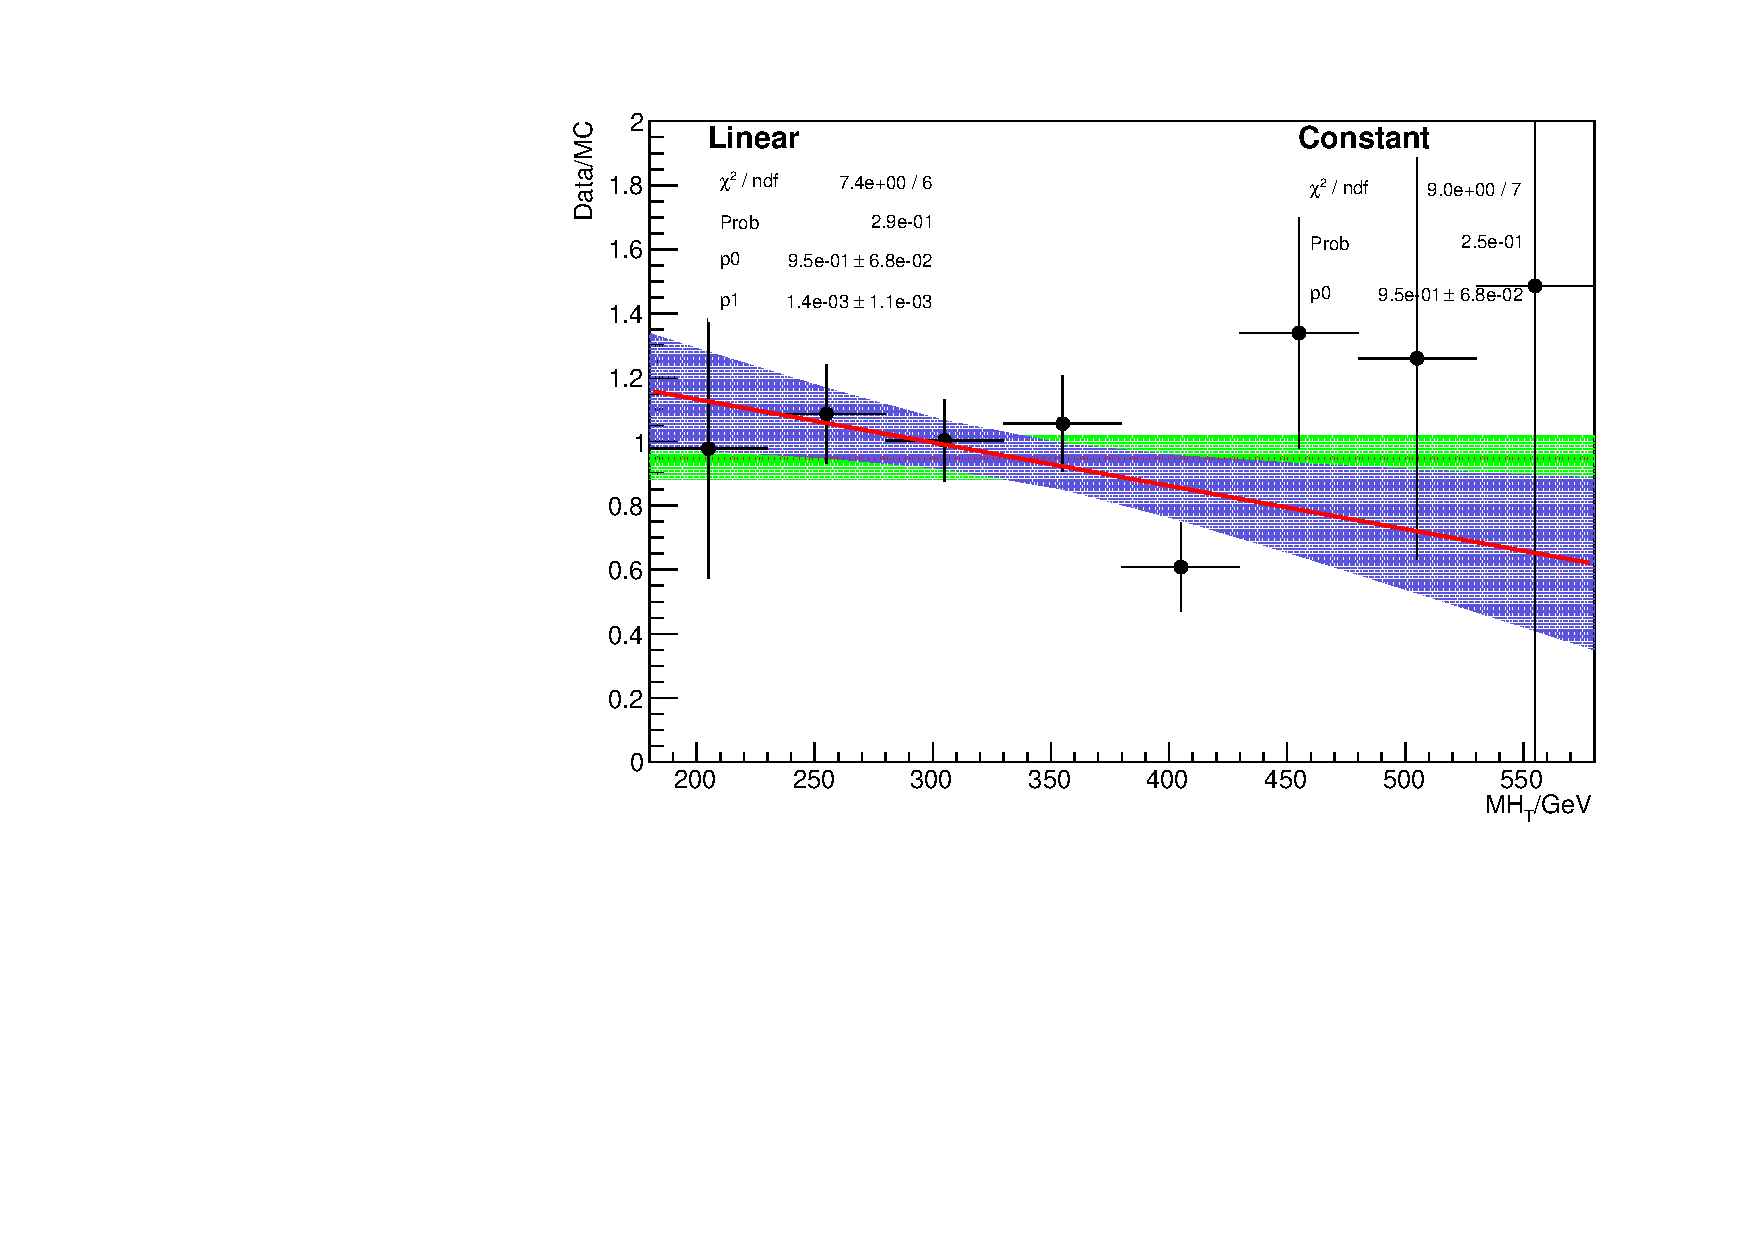
\includegraphics[width=0.5\textwidth]{figures/template/linear/mht_eq0b_ge4j_ht_475_575_SinglePhoton.pdf}
  }~~
  \subfigure[\mmj]{
    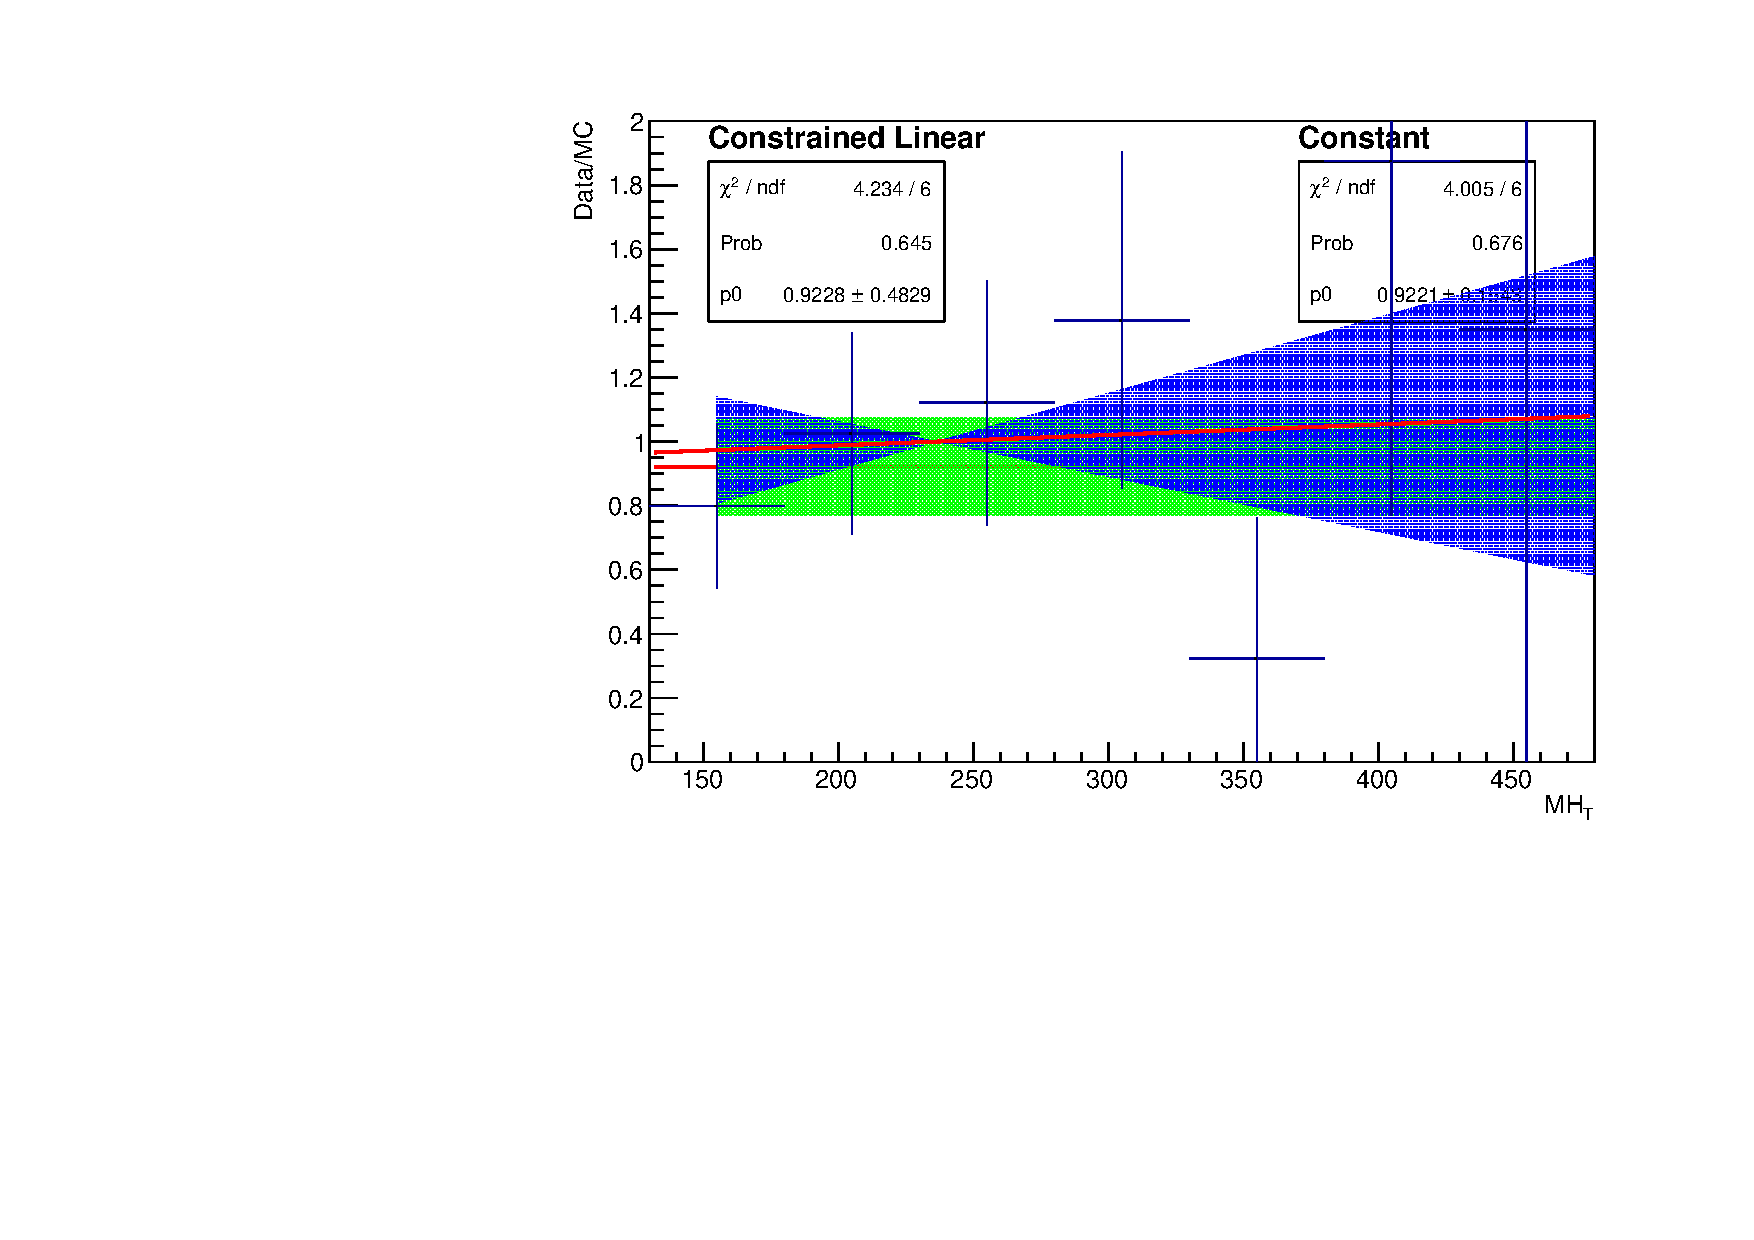
\includegraphics[width=0.5\textwidth]{figures/template/linear/mht_eq0b_ge4j_ht_475_575_DoubleMu.pdf}
  }\\
  \subfigure[\mj]{
    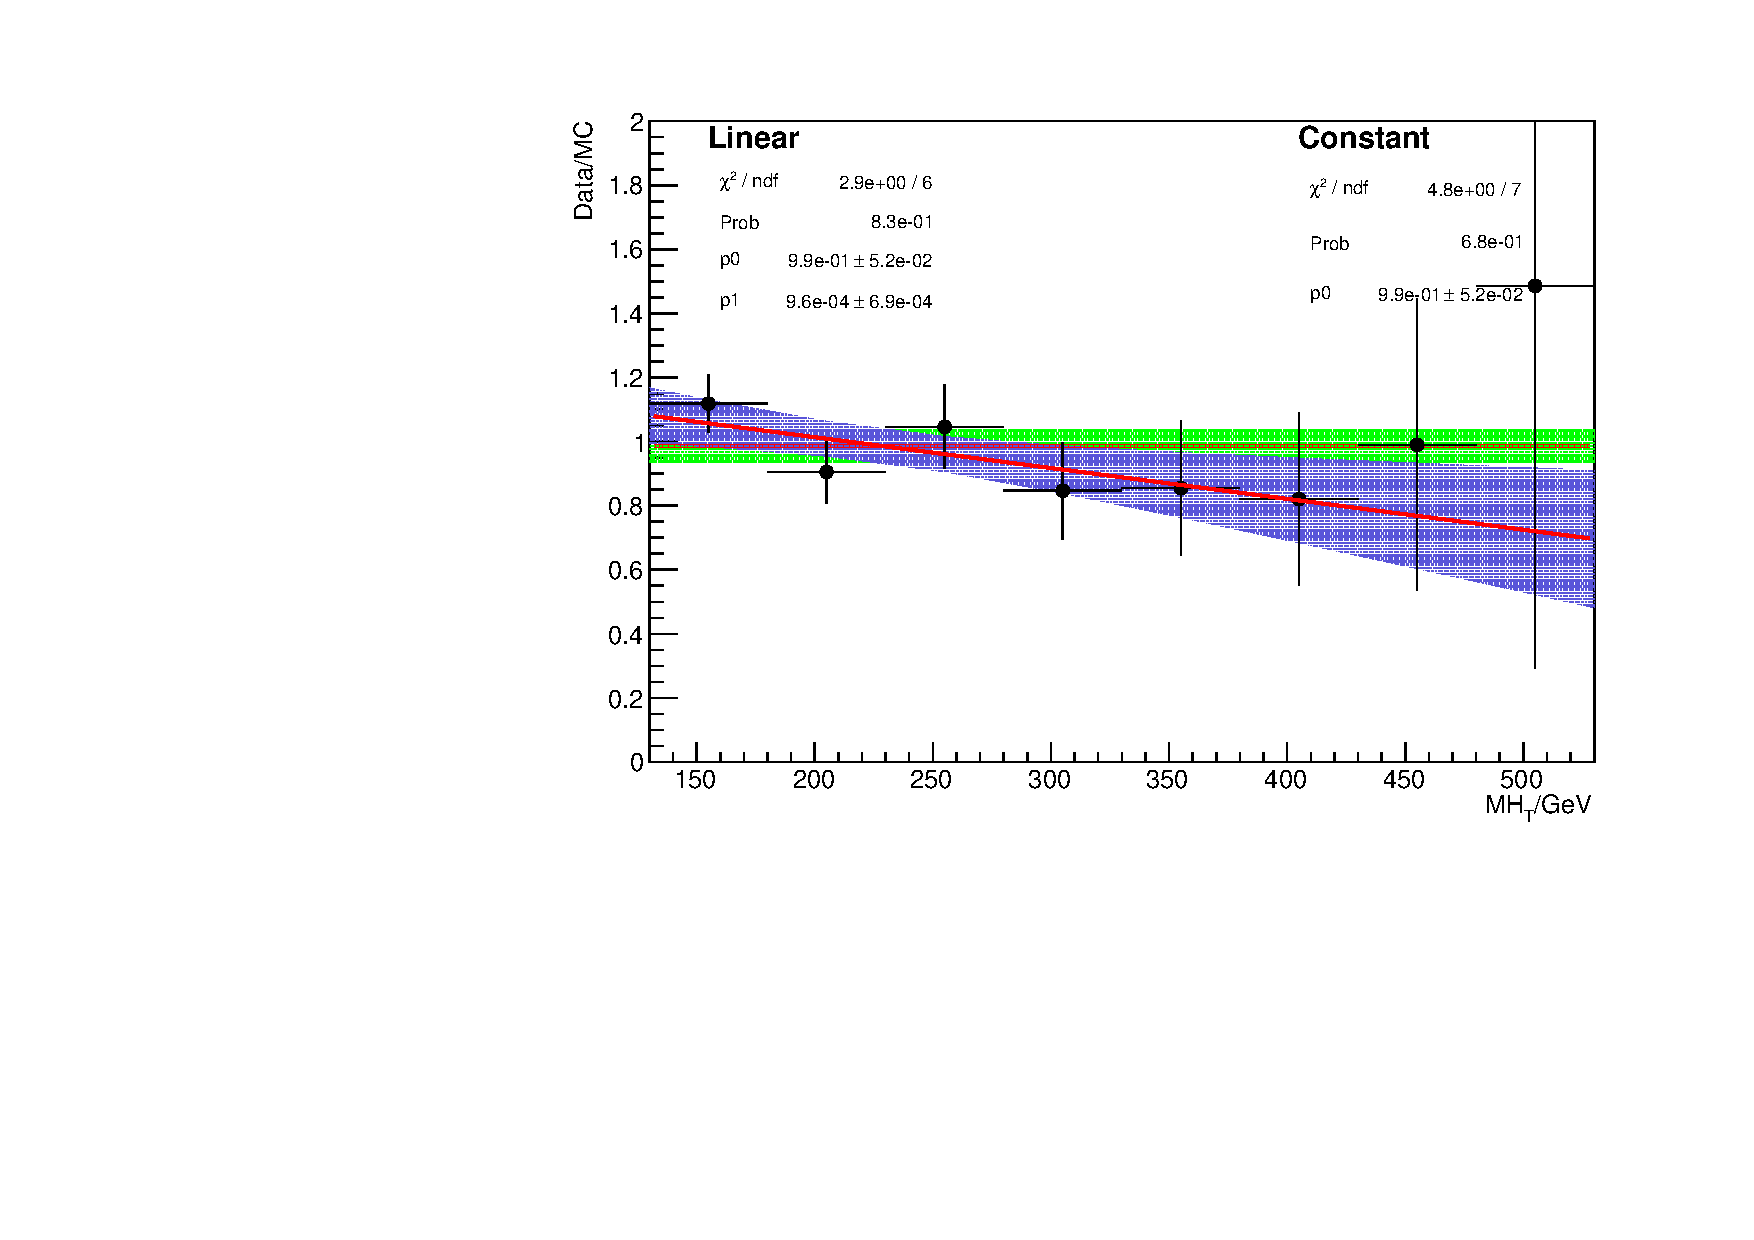
\includegraphics[width=0.5\textwidth]{figures/template/linear/mht_eq0b_ge4j_ht_475_575_SingleMu.pdf}
  }~~
  \\
  \caption{\label{fig:linearFits0bGe4} 
  The data/MC distribution against \mht for the 0b, $\ge4$j category and \scalht 475-575\GeV bin.
  The large linear bias in the linear component seen in Figure~\ref{fig:linearMotiv} is
  largely mitigated.
}
\end{figure}

\begin{figure}[h!]
  \centering
  \subfigure[\gj]{
    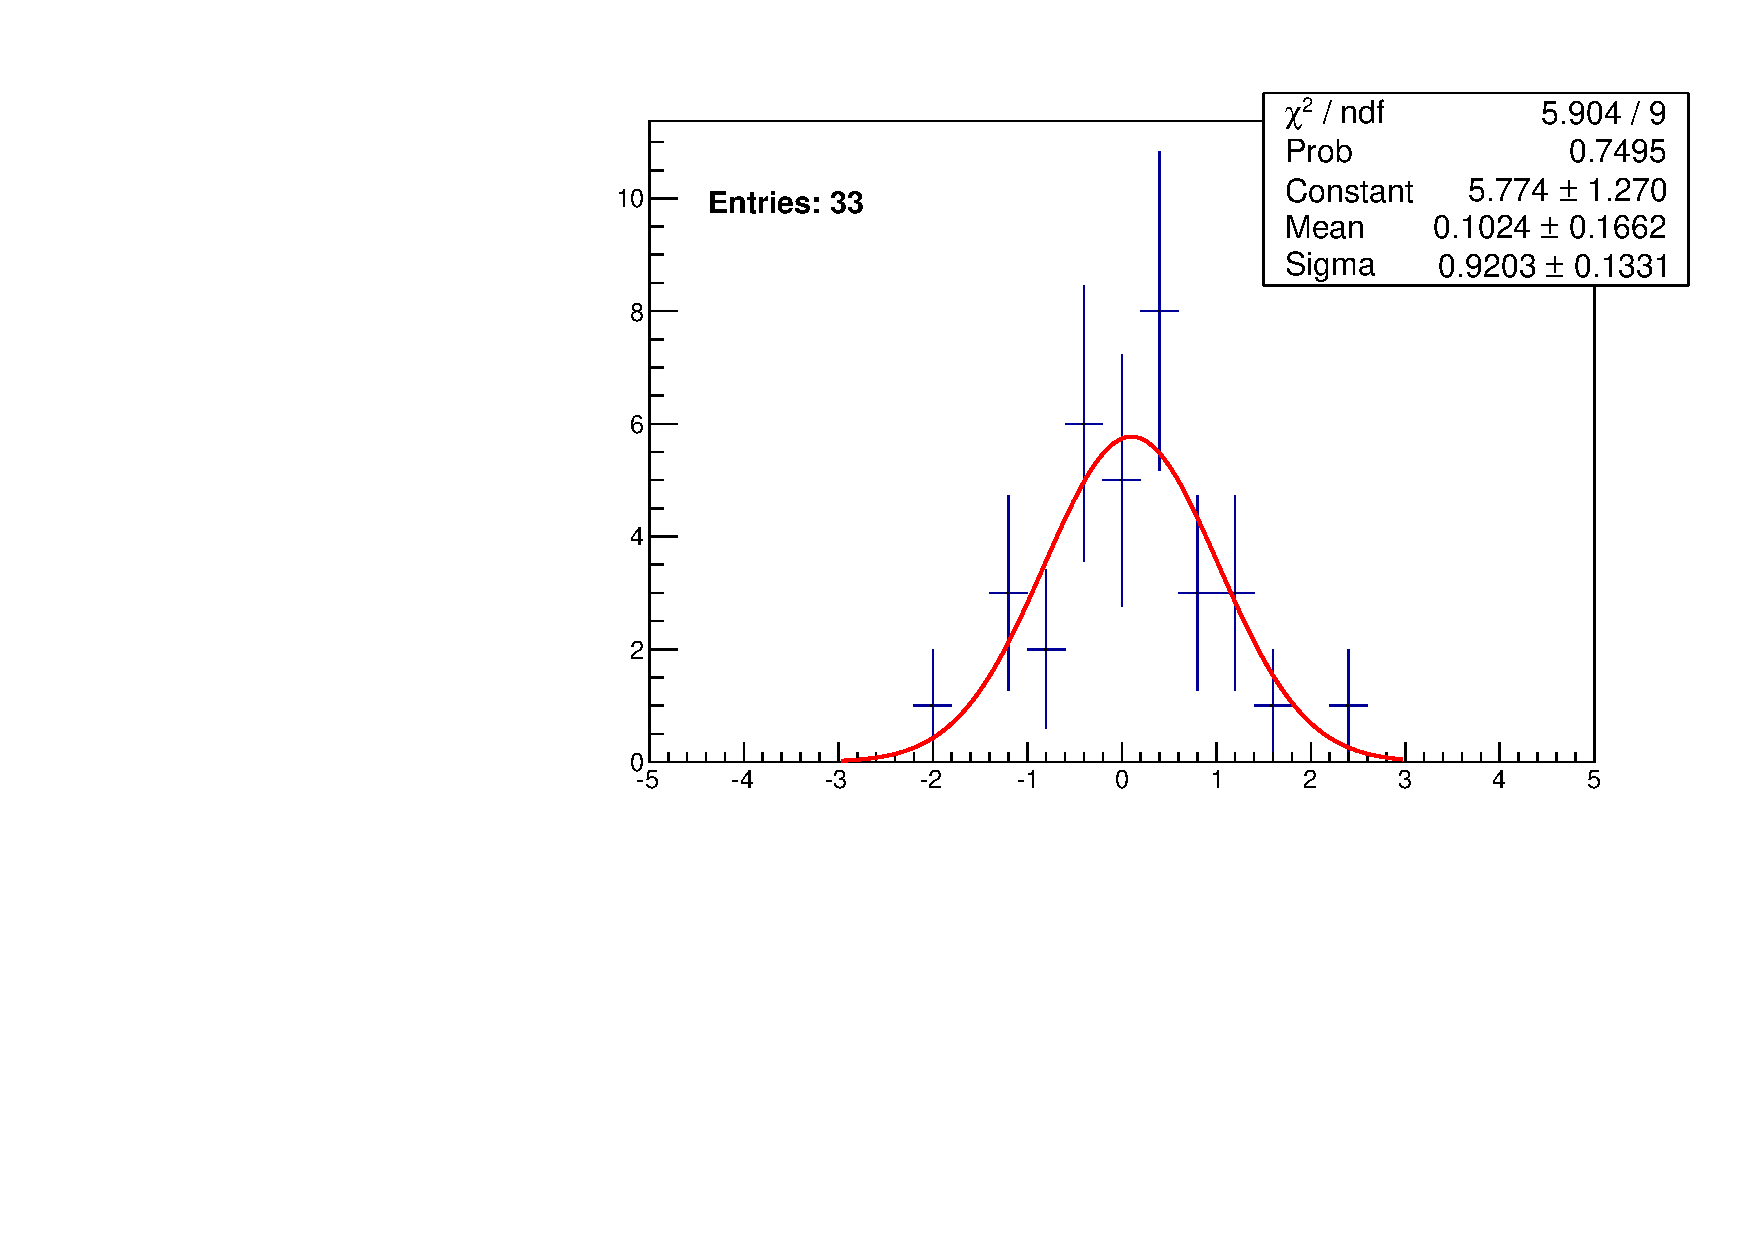
\includegraphics[width=0.5\textwidth]{figures/template/linear/pull_Linear2D_p1_SinglePhoton.pdf}
  }~~
  \subfigure[\mmj]{
    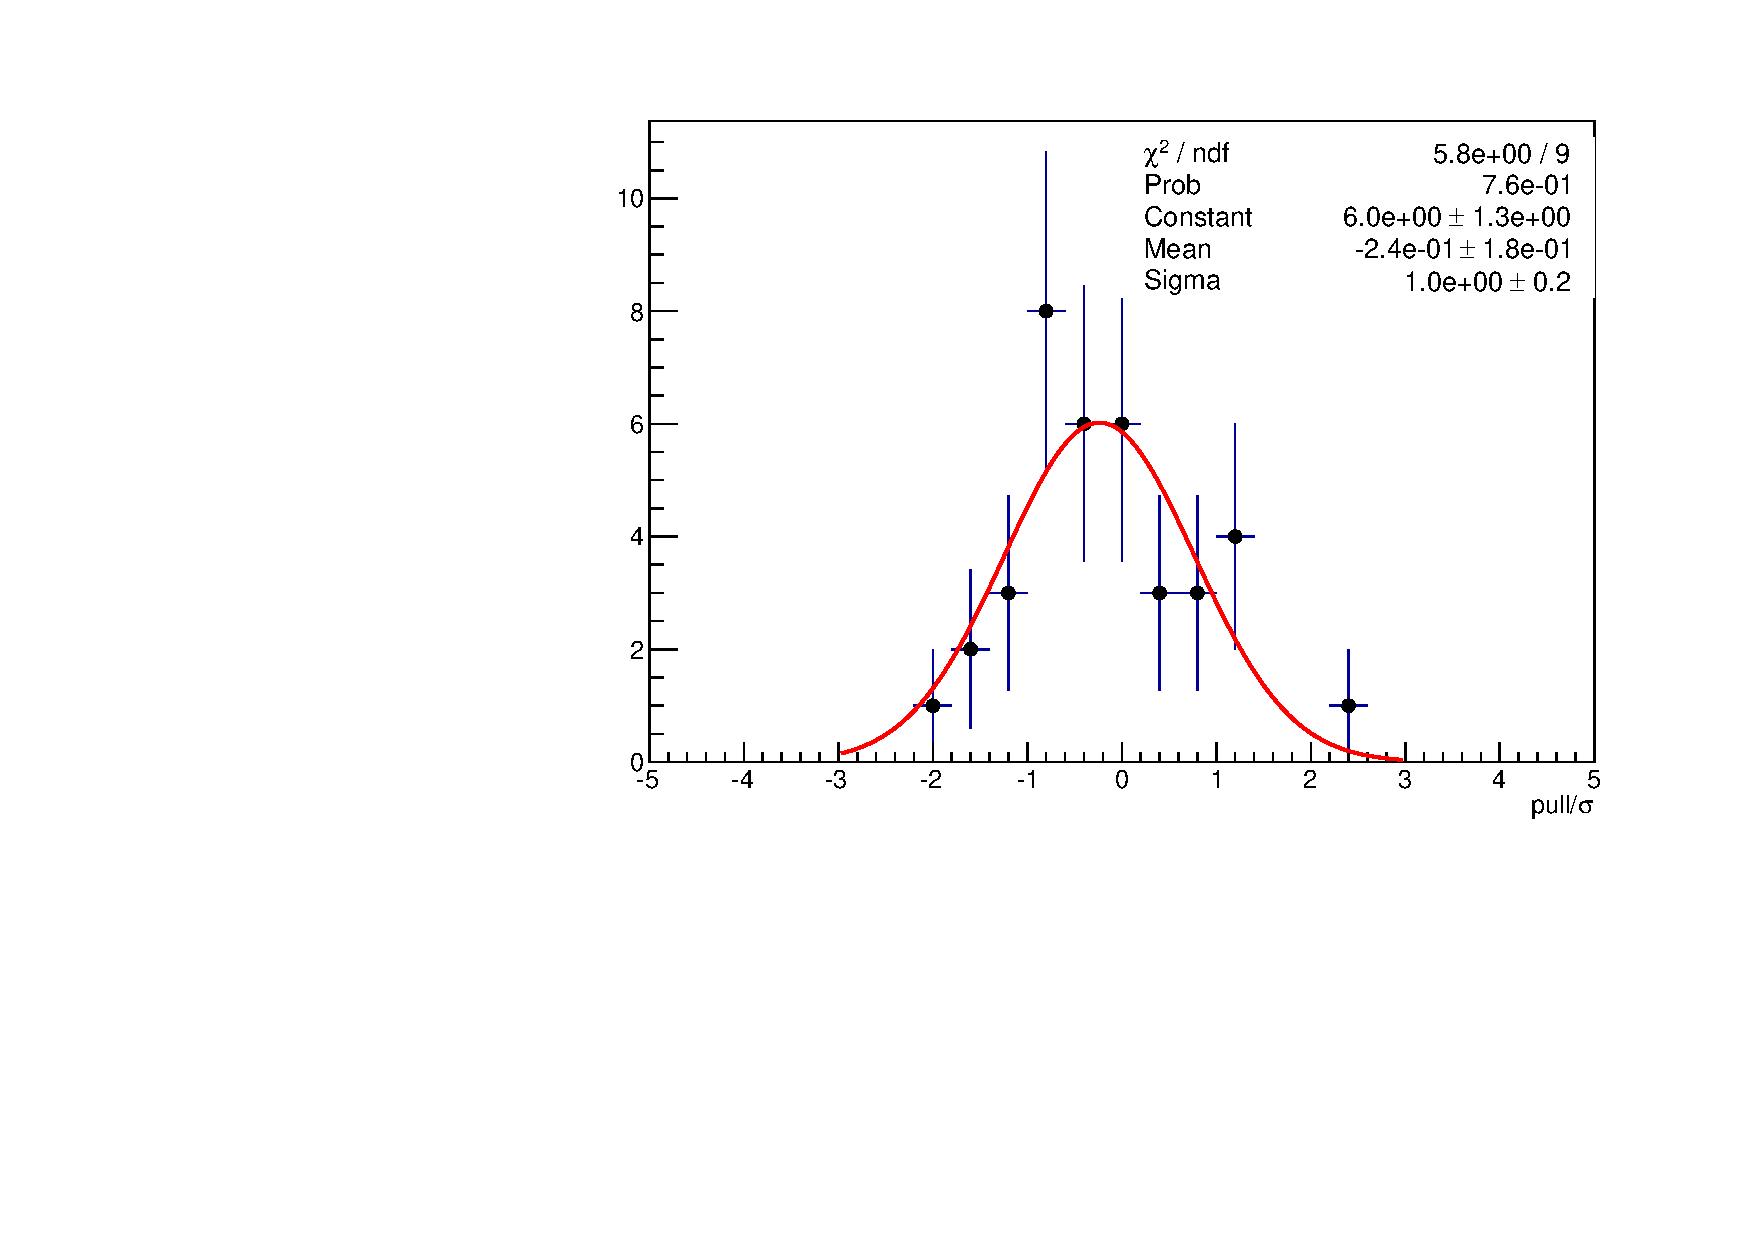
\includegraphics[width=0.5\textwidth]{figures/template/linear/pull_Linear2D_p1_DoubleMu.pdf}
  }\\
  \subfigure[\mj]{
    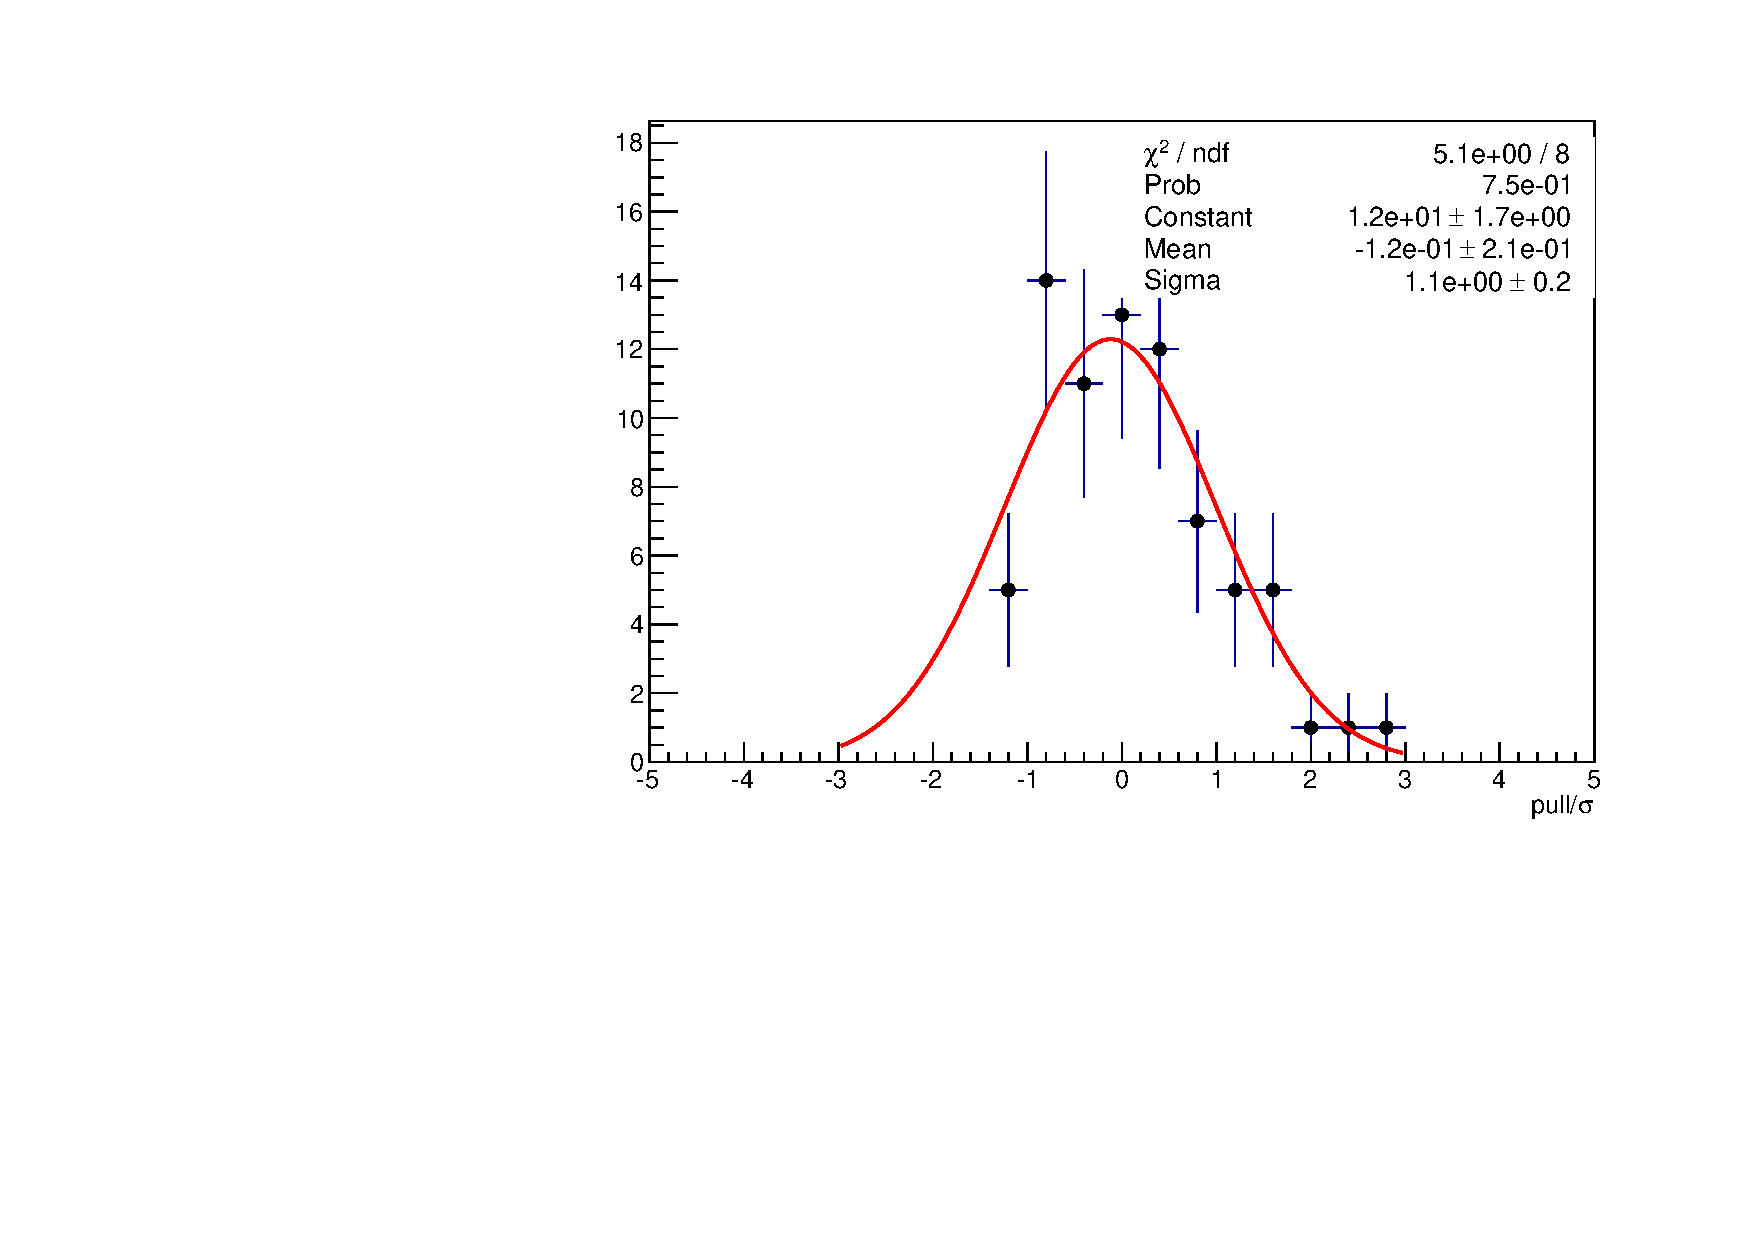
\includegraphics[width=0.5\textwidth]{figures/template/linear/pull_Linear2D_p1_SingleMu.pdf}
  }~~
  \\
  \caption{\label{fig:pulls} 
  The pull distribution of the linear parameter from the flat hypothesis showing
  a distribution consistent with mean and sigma of zero and one. 
  This is consistent with the zero bias hypothesis.
}
\end{figure}
\begin{figure}[h!]
  \centering
  \subfigure[\gj]{
    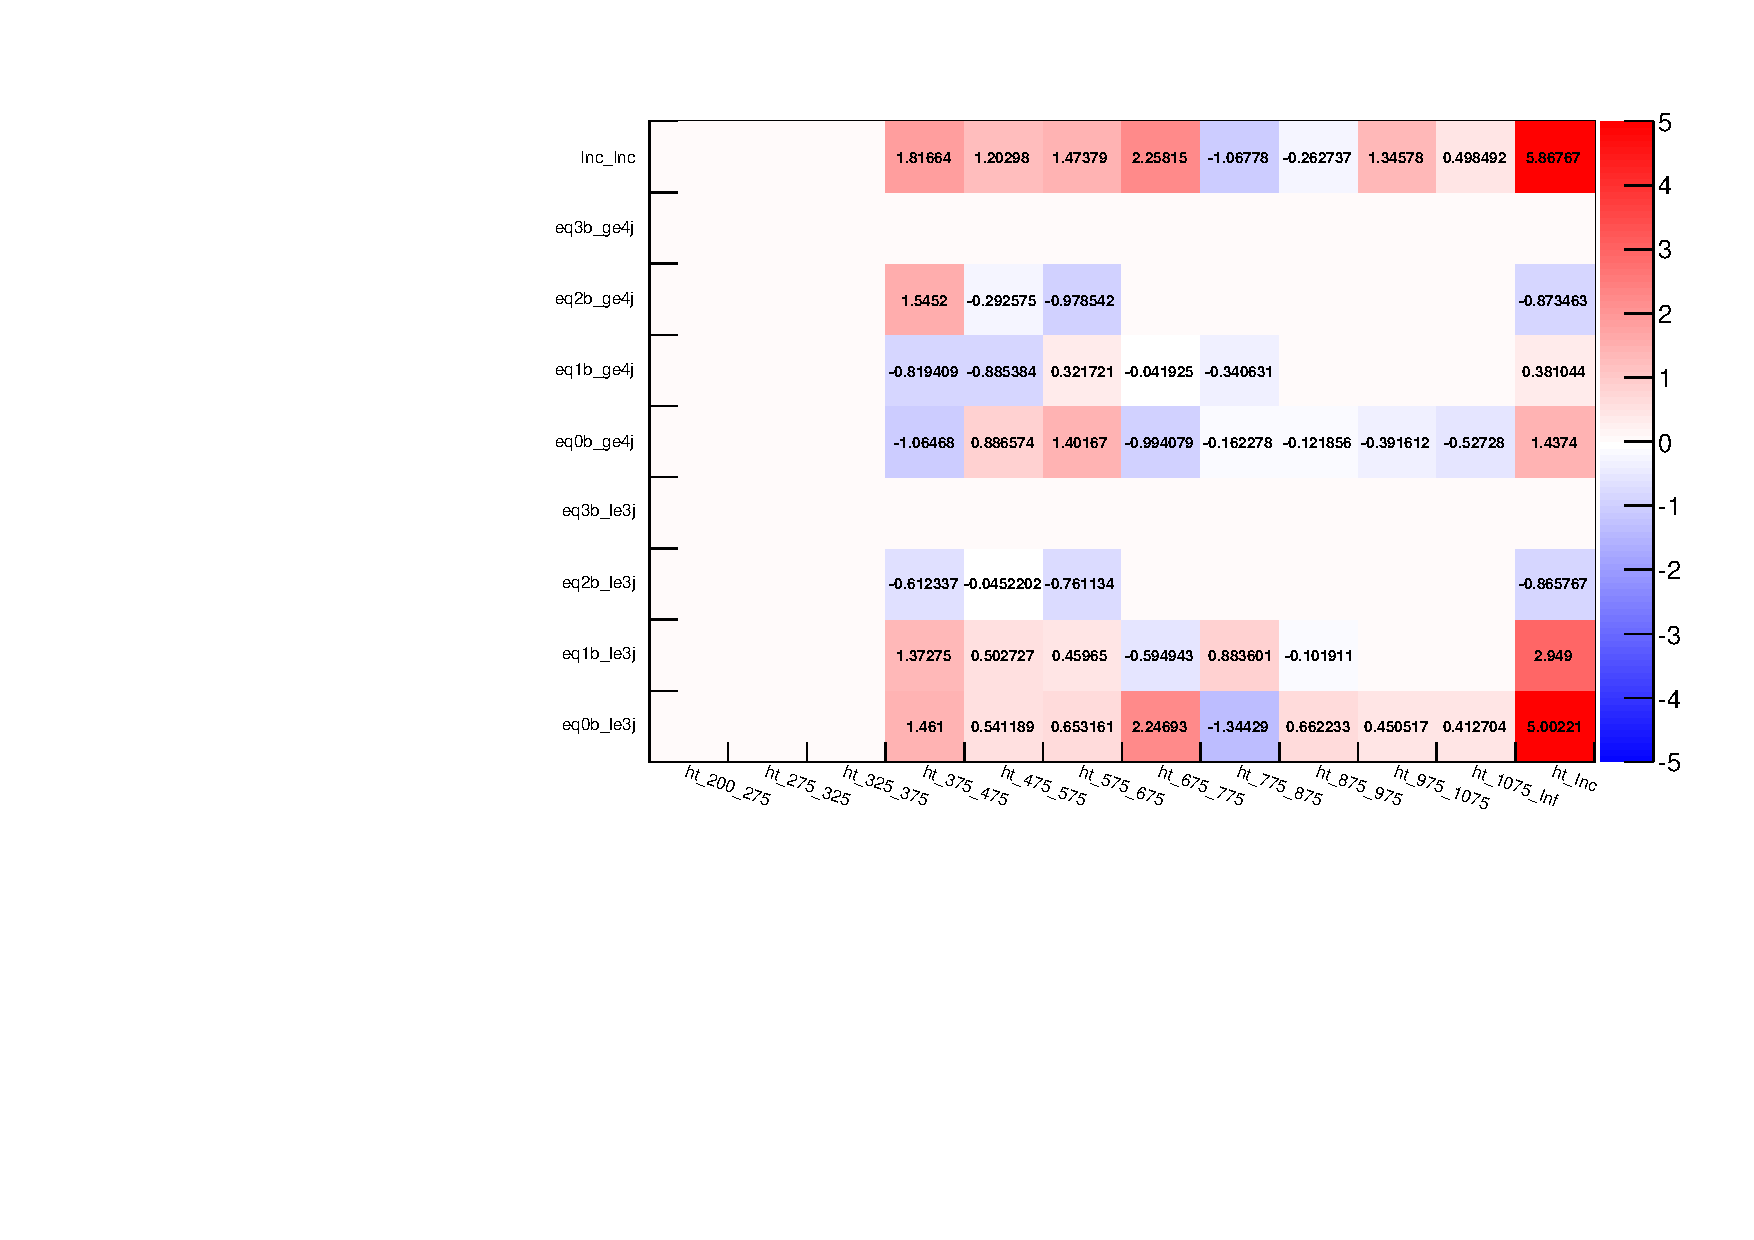
\includegraphics[width=0.5\textwidth]{figures/template/linear/frenchFlagPull_Linear2D_p1_SinglePhoton.pdf}
  }~~
  \subfigure[\mmj]{
    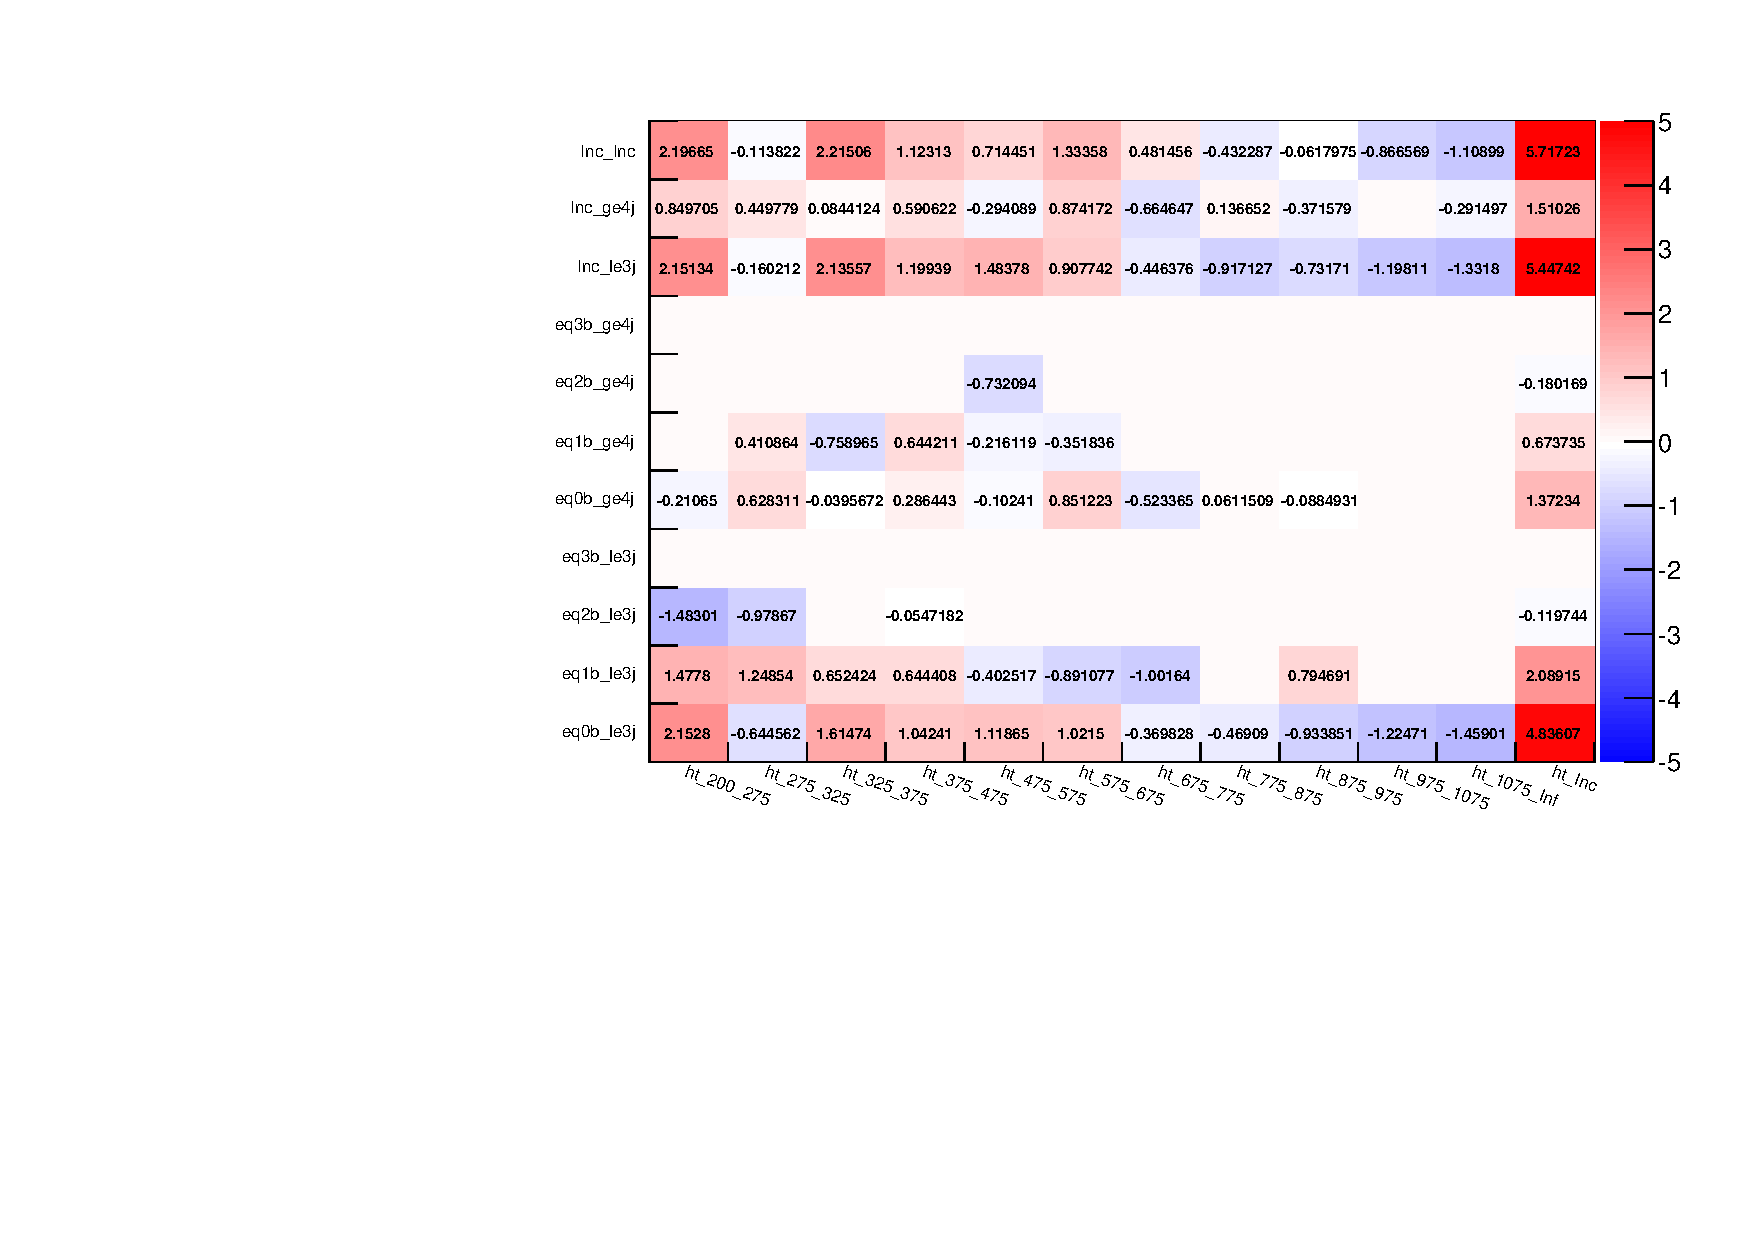
\includegraphics[width=0.5\textwidth]{figures/template/linear/frenchFlagPull_Linear2D_p1_DoubleMu.pdf}
  }\\
  \subfigure[\mj]{
    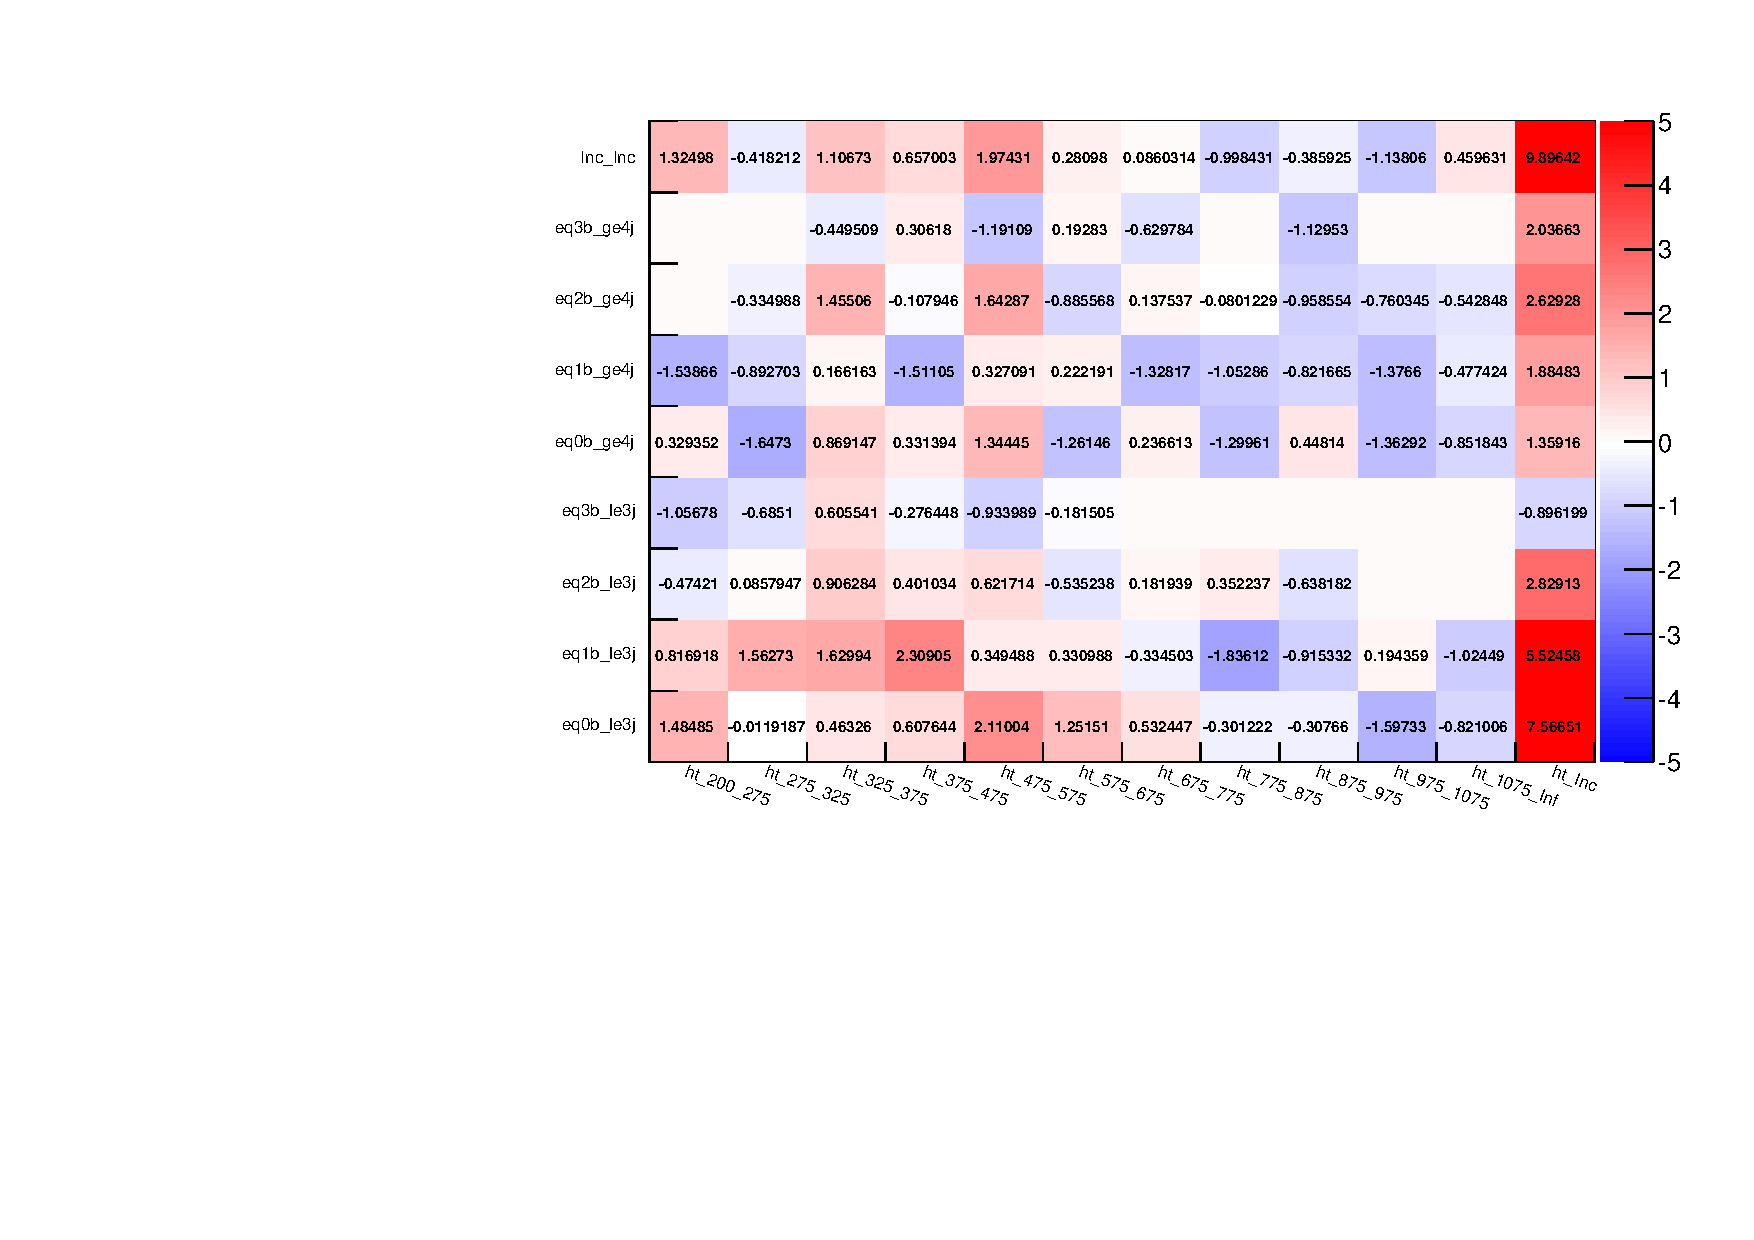
\includegraphics[width=0.5\textwidth]{figures/template/linear/frenchFlagPull_Linear2D_p1_SingleMu.pdf}
  }~~
  \\
  \caption{\label{fig:frenchFlagPulls} 
  The pull distribution of the linear parameter from the flat hypothesis across all
  \scalht bins and categories. There are no significant pulls for the \scalht binned
  fits while the \scalht inclusive case shows very large pulls as expected. 
  Due to trigger requirements the \gj control sample may only be used for \scalht $> 375$\GeV.

}
\end{figure}
\subsection{Deriving systematic on \mht dimension}
\label{sec:systMhtDimension}
The systematic in the \mht dimension is extracting from the hypothesis
of zero bias. The control regions are used to determine the statistical 
precision to which this hypothesis can be confirmed. The procedure for
this is described in this section.

Each background in the signal region (\ttbar/W  and \zInv~) is predicted 
using several control regions. In order to determine an uncertainty in
the \mht dimension a combined fit is made over all relevant control regions
of the linear function. The uncertainty on the linear parameter is then
used to define the up and down one sigma variations of the nominal template.
As a conservative estimate the difference from zero is added in quadrature
to the uncertainty on the linear parameter and used to define the overall
uncertainty on the parameter. 

The result from using such a template is shown in Figure~\ref{fig:signalOverlay} where the 
template variations for both relevant backgrounds have been combined
to show the overall uncertainty on the \mht dimension. This is tested using data from
the 8 \TeV signal region where no signal contribution is expected. The data scatter
in the signal region is overlain for several bins and categories 
to show variations consistent within the expected uncertainty from the control regions.

An additional validation is carried out by comparing the expected and observed uncertainties
on the linear parameter defining the template variations.
The expected errors are derived by using a linear fit to the MC/MC ratio where the numerator
have errors given by the poisson uncertainty on the number of predicted counts while
the uncertainty on the denominator comes from the statistical uncertainty on the
MC prediction. The relative errors derived from this approach for \ttbar/W and \zInv~ are shown in 
Figure~\ref{fig:expectedObservedTtw} and Figure~\ref{fig:expectedObservedZinv} 
and compared to the observed relative uncertainties. These show good agreement 
which provides additional motivation for the zero bias hypothesis as
well as validating the method for deriving expected uncertainties.


\begin{figure}[h!]
  \centering
  \subfigure[Category 0b, $\le3$j and $\scalht$ $375-475$ \GeV]{
    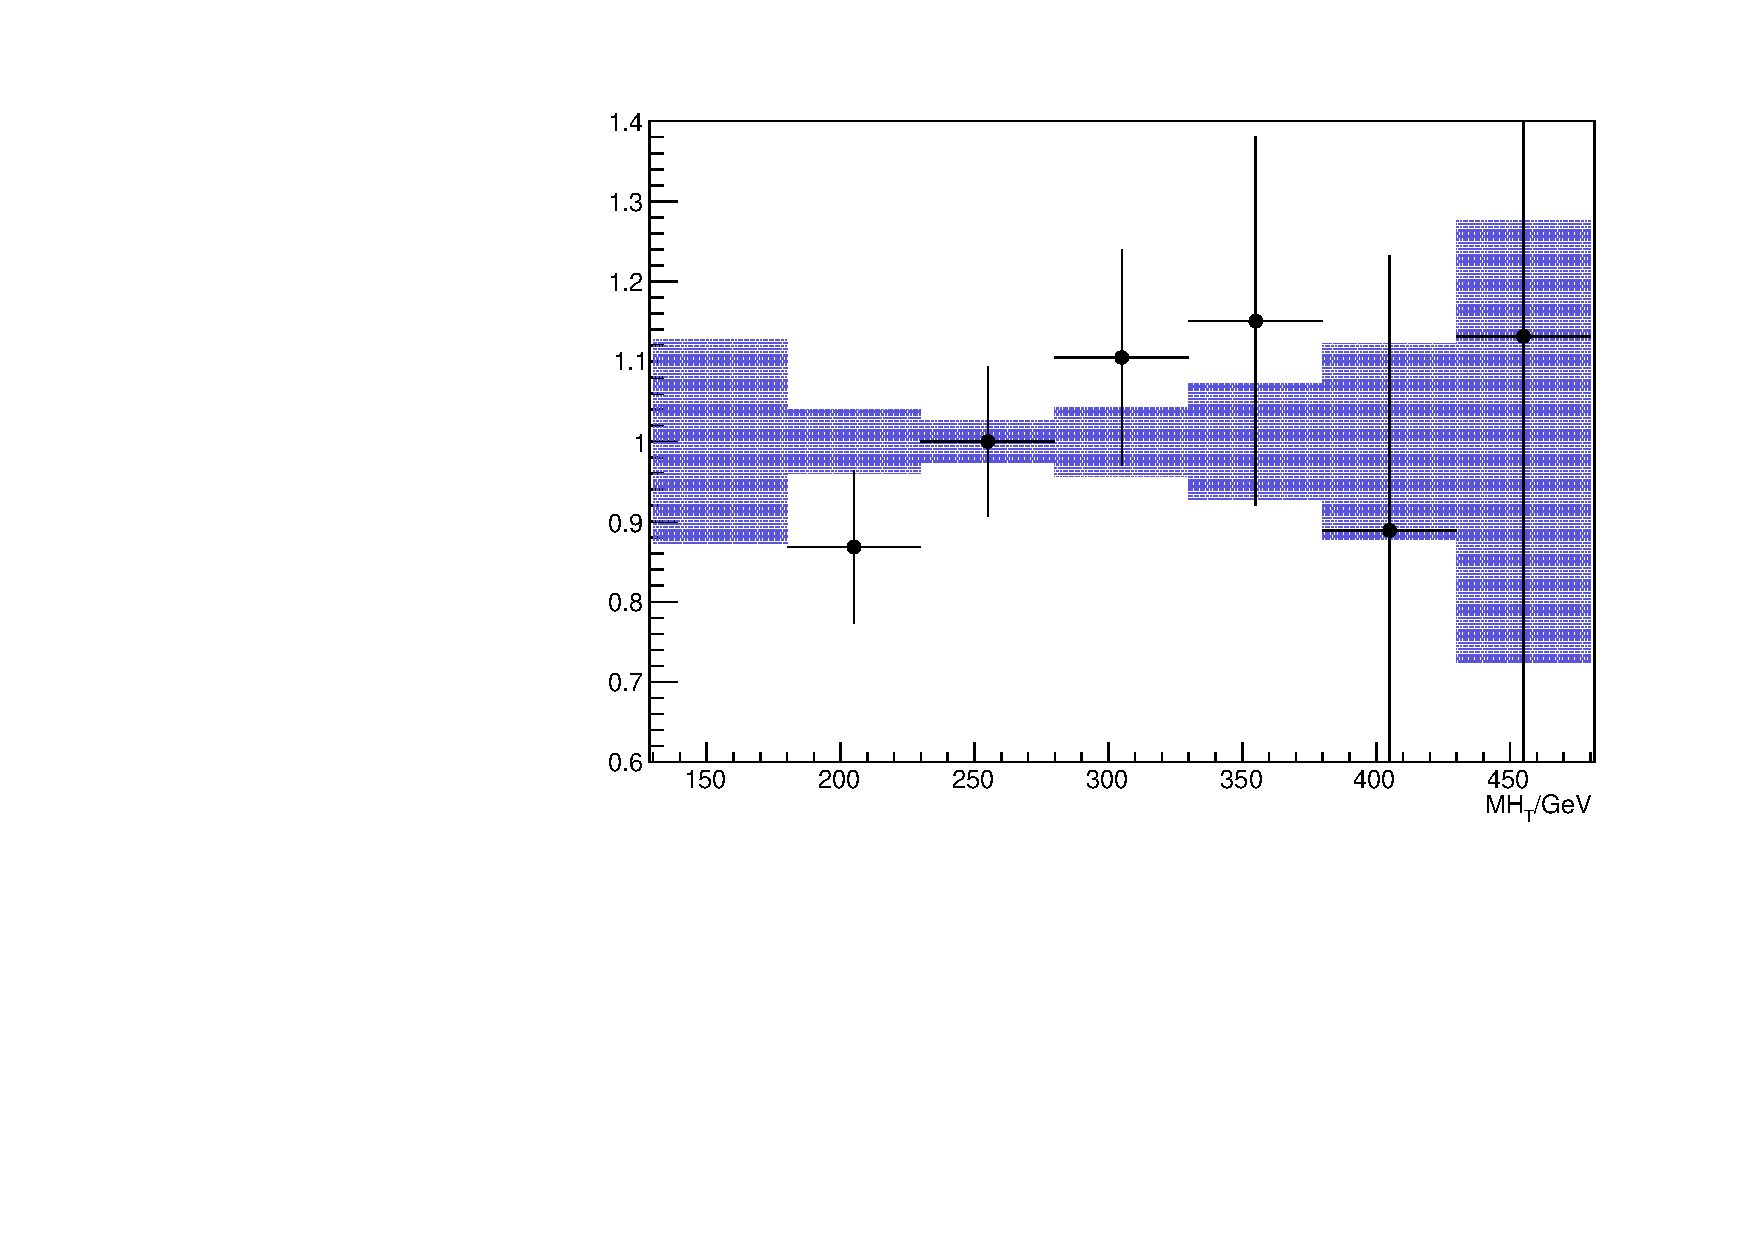
\includegraphics[width=0.5\textwidth]{figures/template/linear/mht_eq0b_ge4j_ht_375_475_MEGA.pdf}
  }~~
  \subfigure[Category 1b, $\le3$j and $\scalht$ $375-475$ \GeV]{
    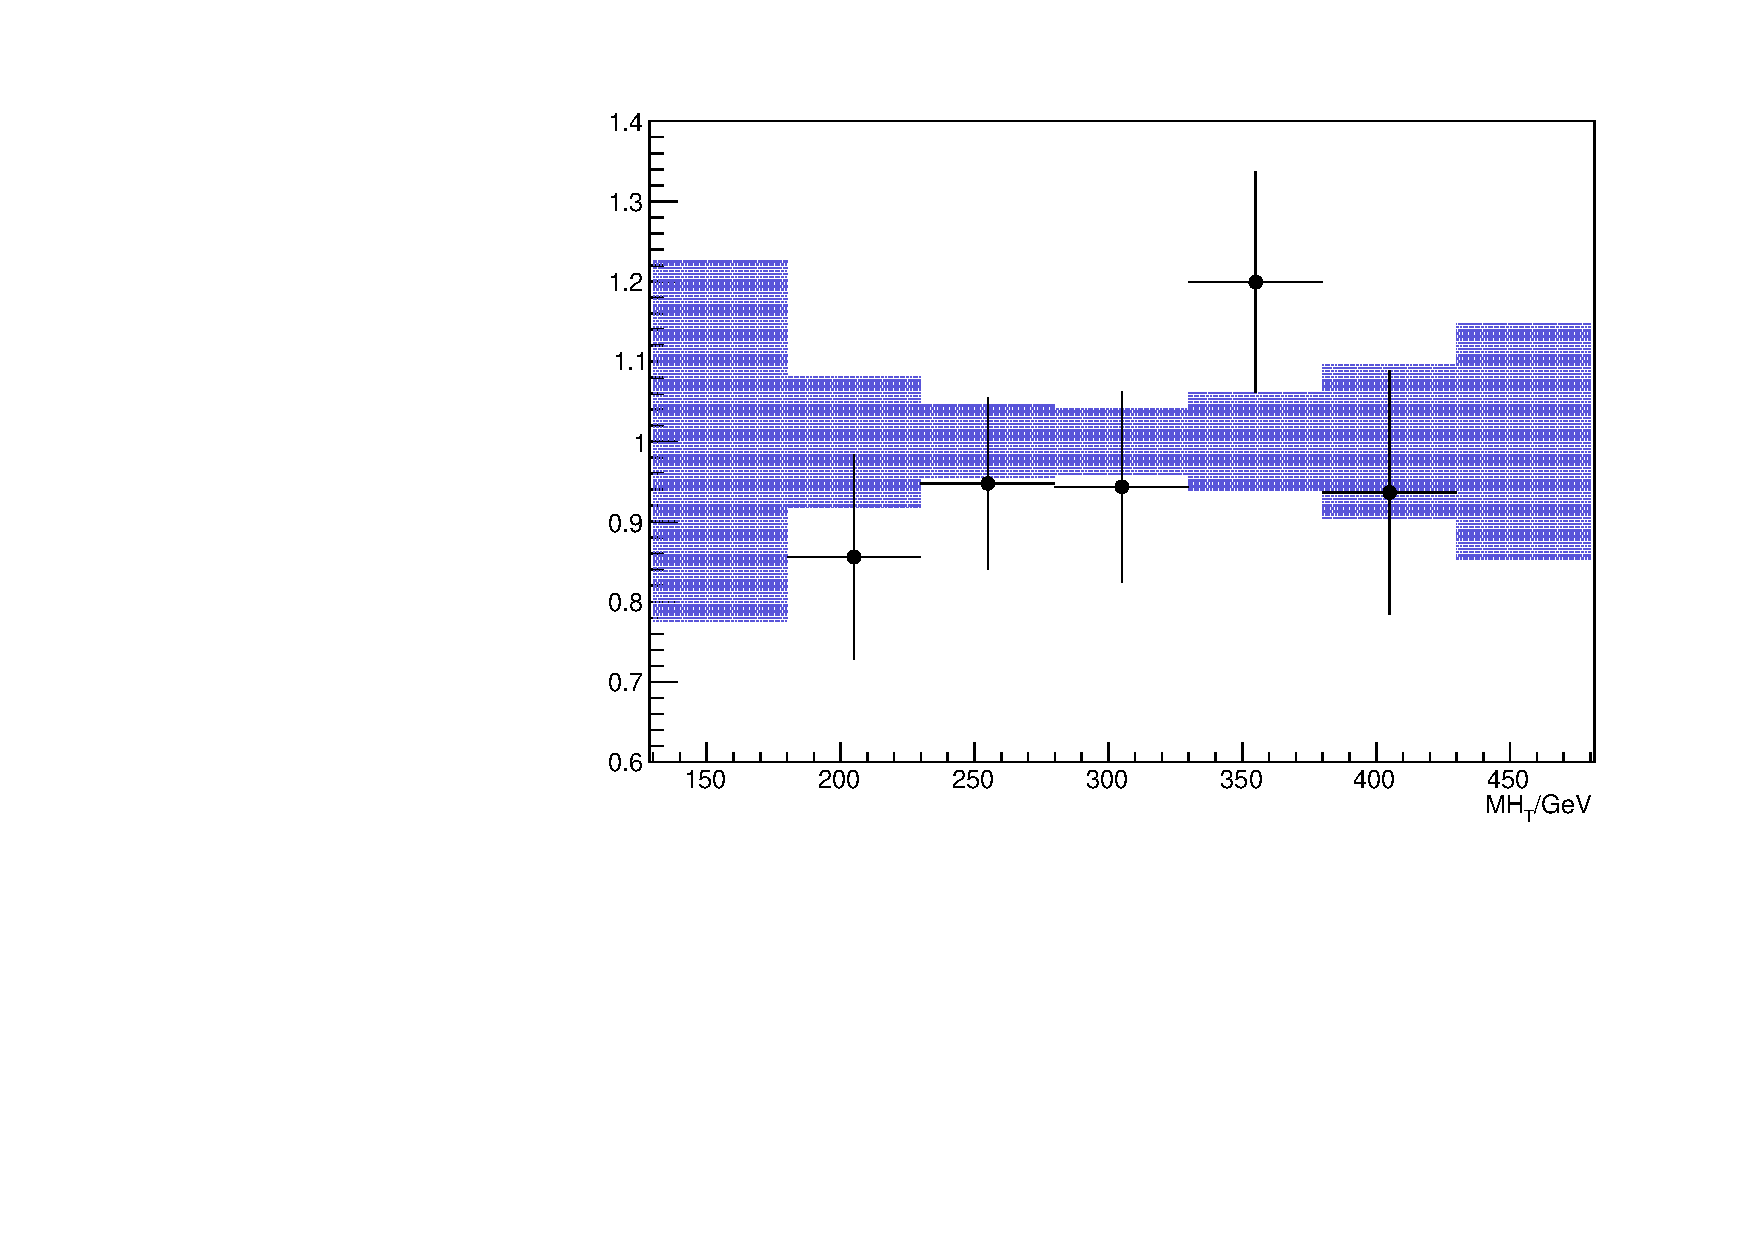
\includegraphics[width=0.5\textwidth]{figures/template/linear/mht_eq1b_le3j_ht_375_475_MEGA.pdf}
  }\\
  \subfigure[Category 0b, $\ge4$j and $\scalht$ $375-475$ \GeV]{
    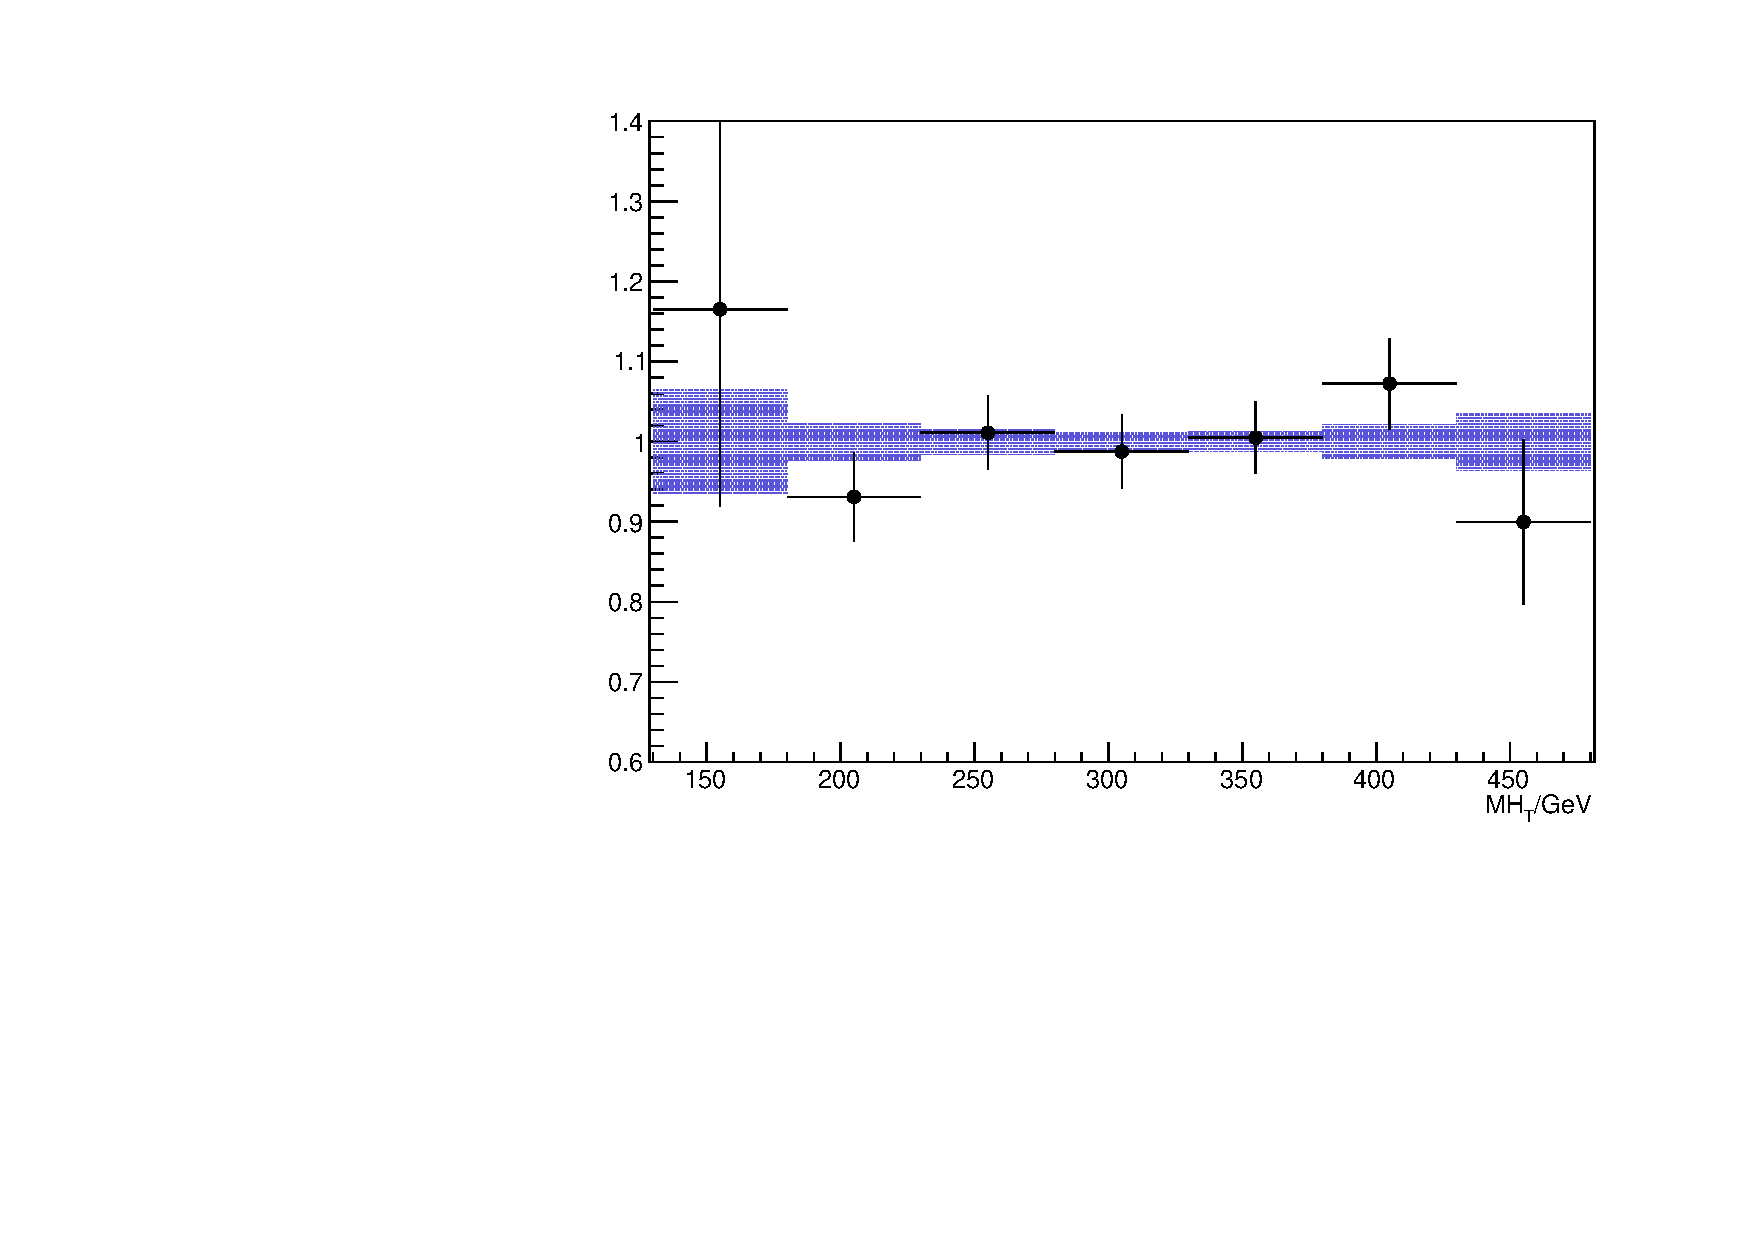
\includegraphics[width=0.5\textwidth]{figures/template/linear/mht_eq0b_le3j_ht_375_475_MEGA.pdf}
  }~~
  \subfigure[Category 0b, $\le3$j and $\scalht$ $475-575$ \GeV]{
    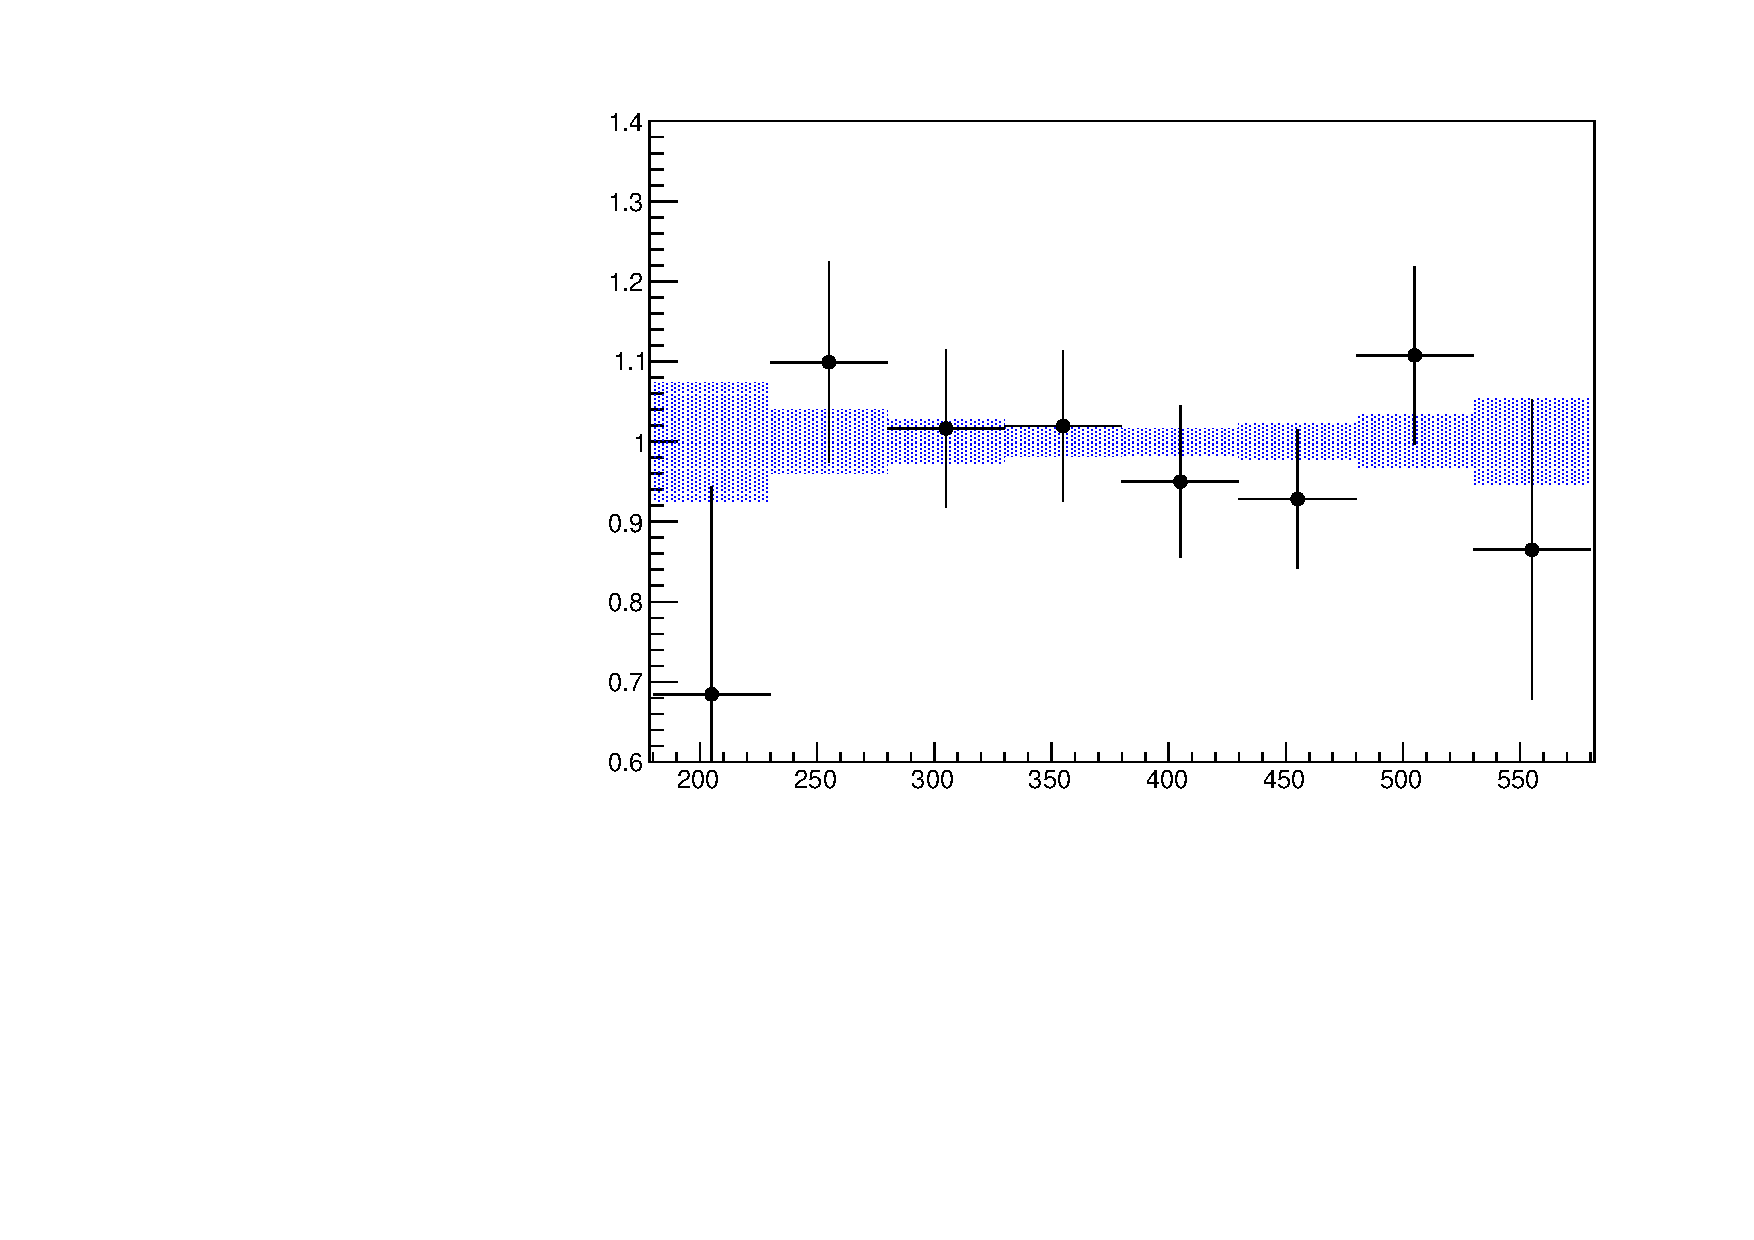
\includegraphics[width=0.5\textwidth]{figures/template/linear/mht_eq0b_le3j_ht_475_575_MEGA.pdf}
  }~~
  \\
  \caption{\label{fig:signalOverlay} 
}
\end{figure}

\begin{figure}[h!]
  \centering
  \subfigure[\label{fig:expectedTtw} Expected uncertainties]{
    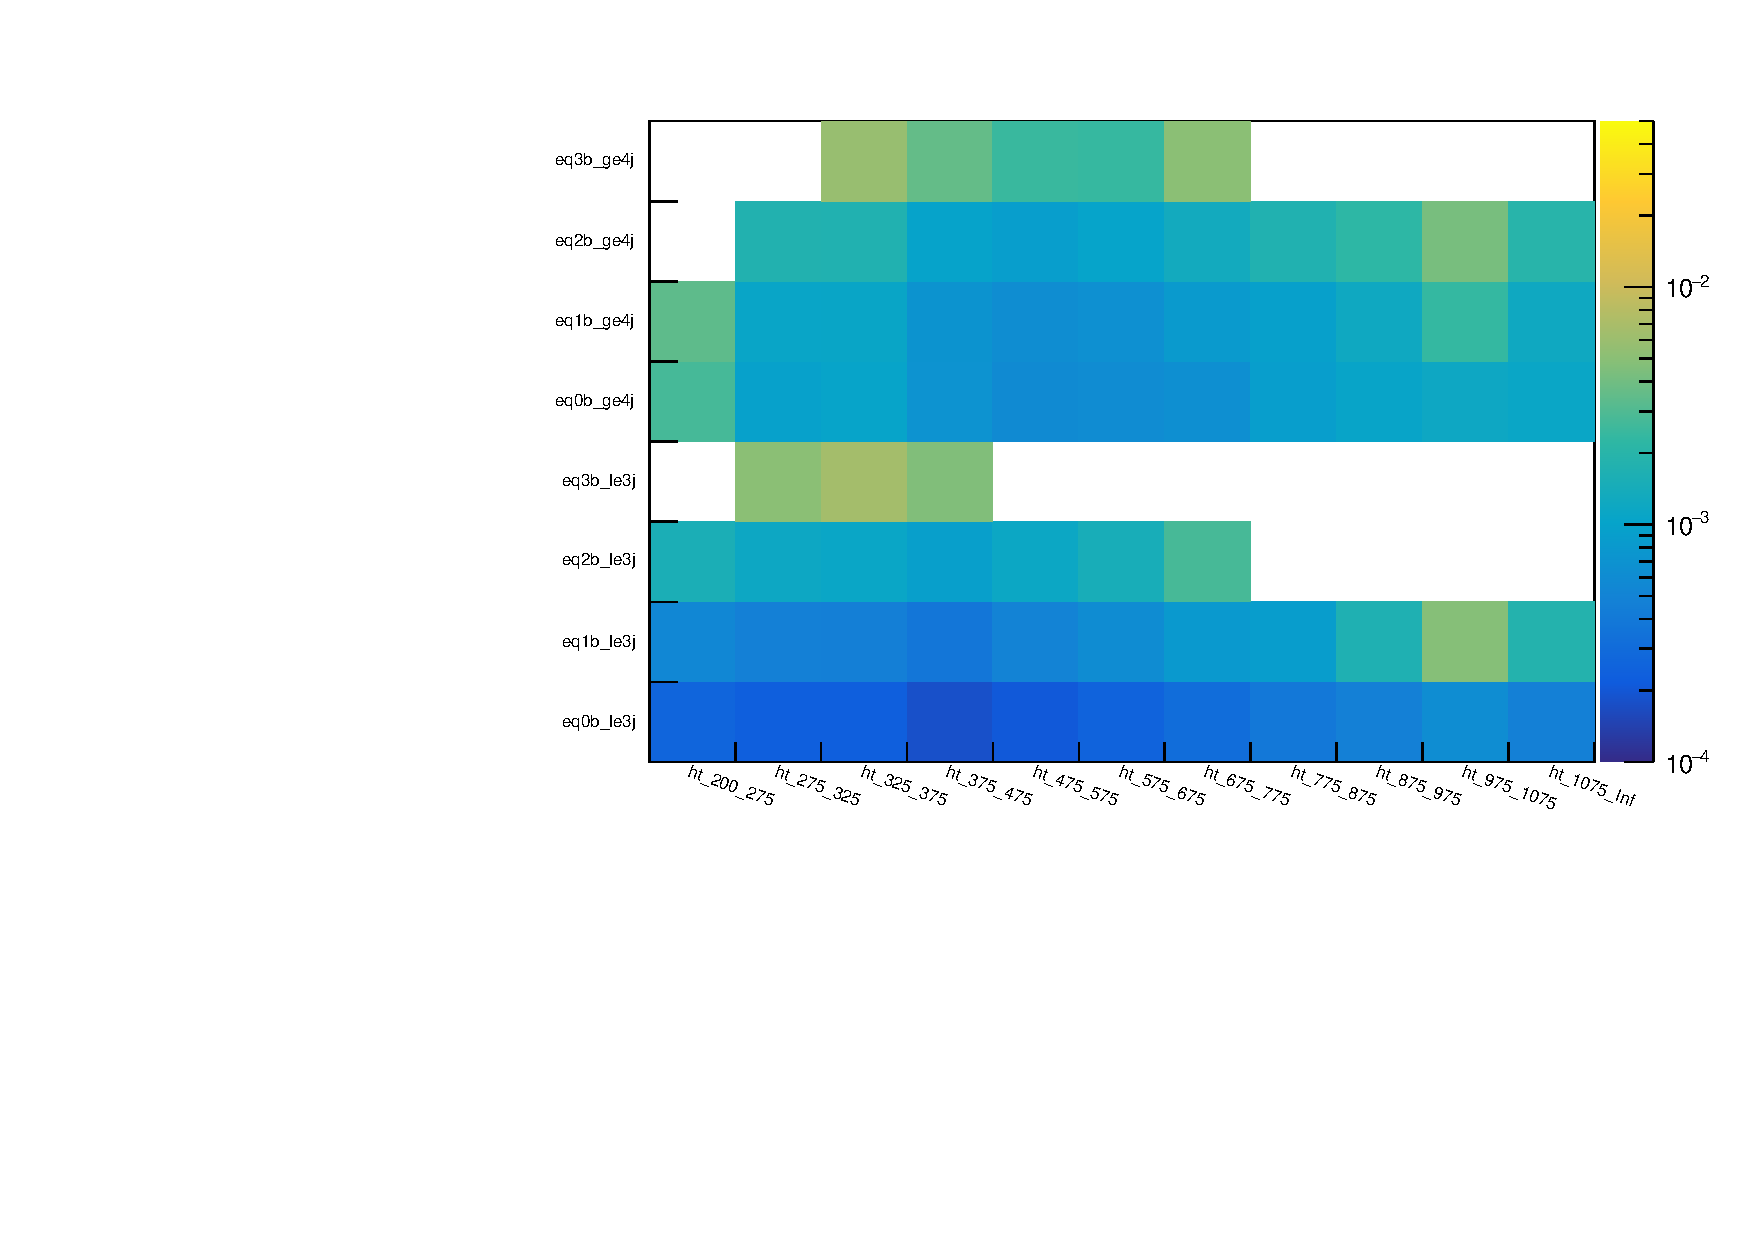
\includegraphics[width=0.5\textwidth]{figures/template/linear/frenchFlagErrCompleteExpected_Linear2D_p1_Ttw.pdf}
  }~~
  \subfigure[\label{fig:observedTtw} Observed uncertainties]{
    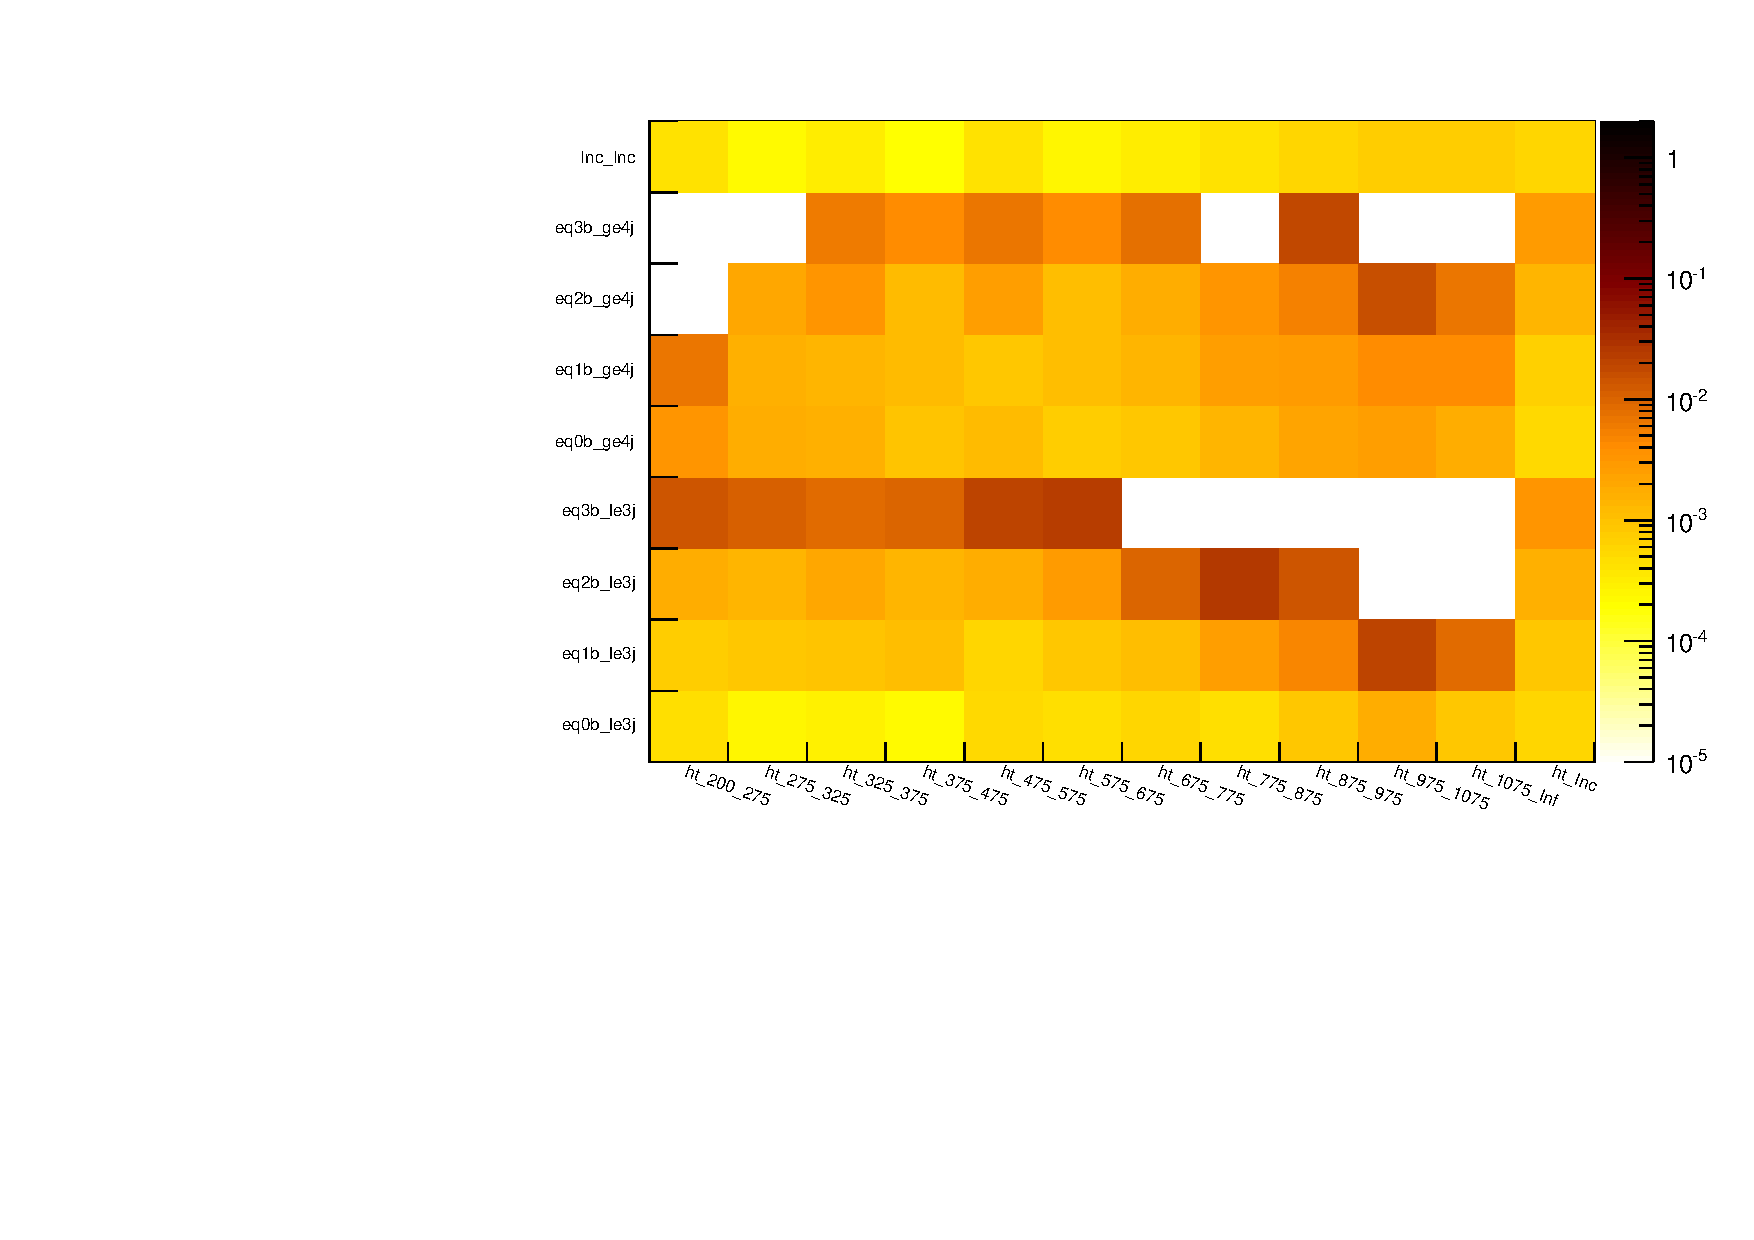
\includegraphics[width=0.5\textwidth]{figures/template/linear/frenchFlagErrComplete_Linear2D_p1_Ttw.pdf}
  }\\
  \caption{\label{fig:expectedObservedTtw}
  Expected relative uncertainties shown for \ttbar/W in Figure~\ref{fig:expectedTtw} are consistent
  with observed relative uncertainties shown in Figure~\ref{fig:observedTtw}.}
\end{figure}

\begin{figure}[h!]
  \centering
  \subfigure[\label{fig:expectedZinv} Expected uncertainties]{
    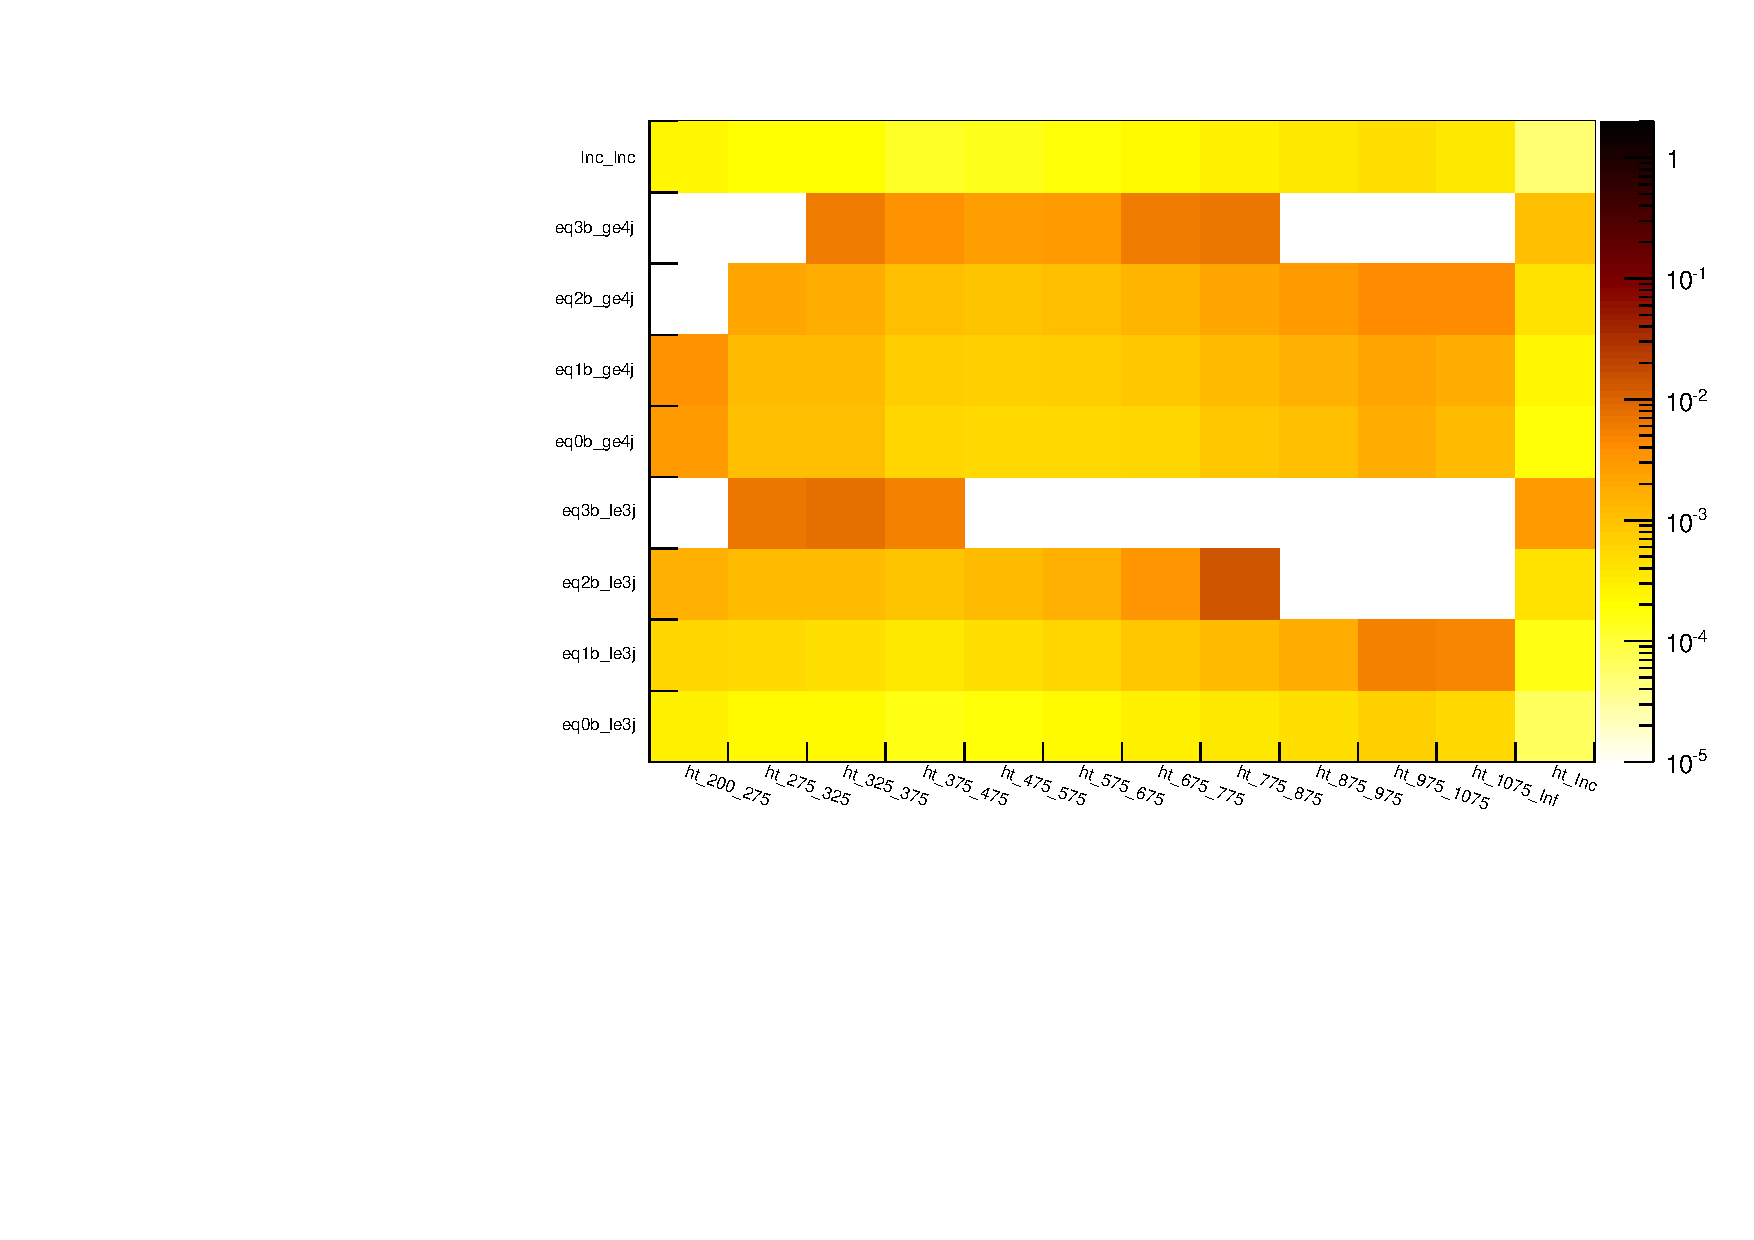
\includegraphics[width=0.5\textwidth]{figures/template/linear/frenchFlagErrCompleteExpected_Linear2D_p1_Zinv.pdf}
  }~~
  \subfigure[\label{fig:observedZinv} Observed uncertainties]{
    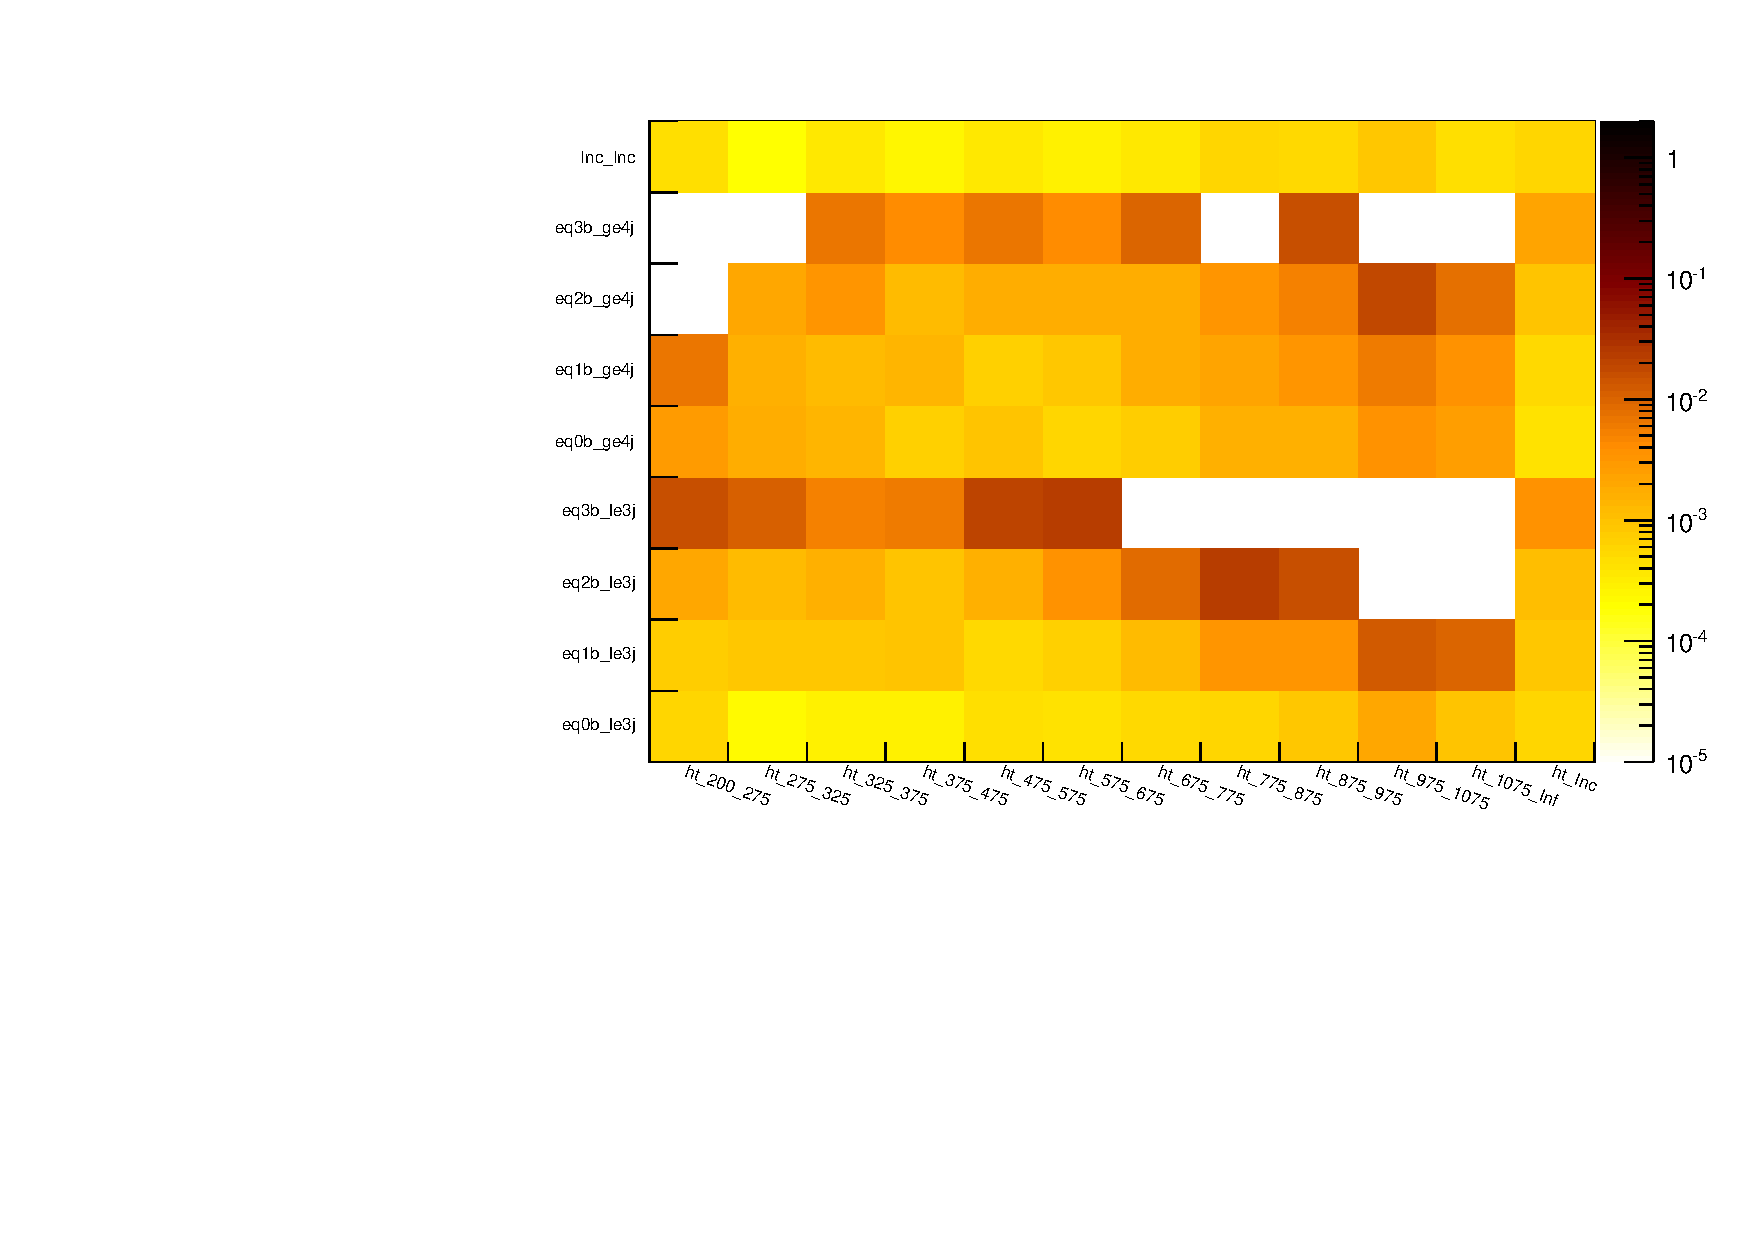
\includegraphics[width=0.5\textwidth]{figures/template/linear/frenchFlagErrComplete_Linear2D_p1_Zinv.pdf}
  }\\
  \caption{\label{fig:expectedObservedZinv}
  Expected relative uncertainties shown for \zInv~ in Figure~\ref{fig:expectedZinv} are consistent
  with observed relative uncertainties shown in Figure~\ref{fig:observedZinv}.}
\end{figure}

\subsection{Application to 13 \TeV}
\label{sec:syst13TeV}
Using the method described in Section~\ref{sec:systMhtDimension} the expected uncertainties
from 13 \TeV MC for both \ttbar/W  and \zInv~ using all relevant control regions are
shown in Figure~\ref{fig:expected13}. 
Depending on the category and \scalht bin, uncertainties between 1 and 10\% are found.
An example of the overall uncertainties on the \mht templates is shown
in Figure~\ref{fig:exampleTemplate13}.

\begin{figure}[h!]
  \centering
  \subfigure[\label{fig:ttw13} \ttbar/W]{
    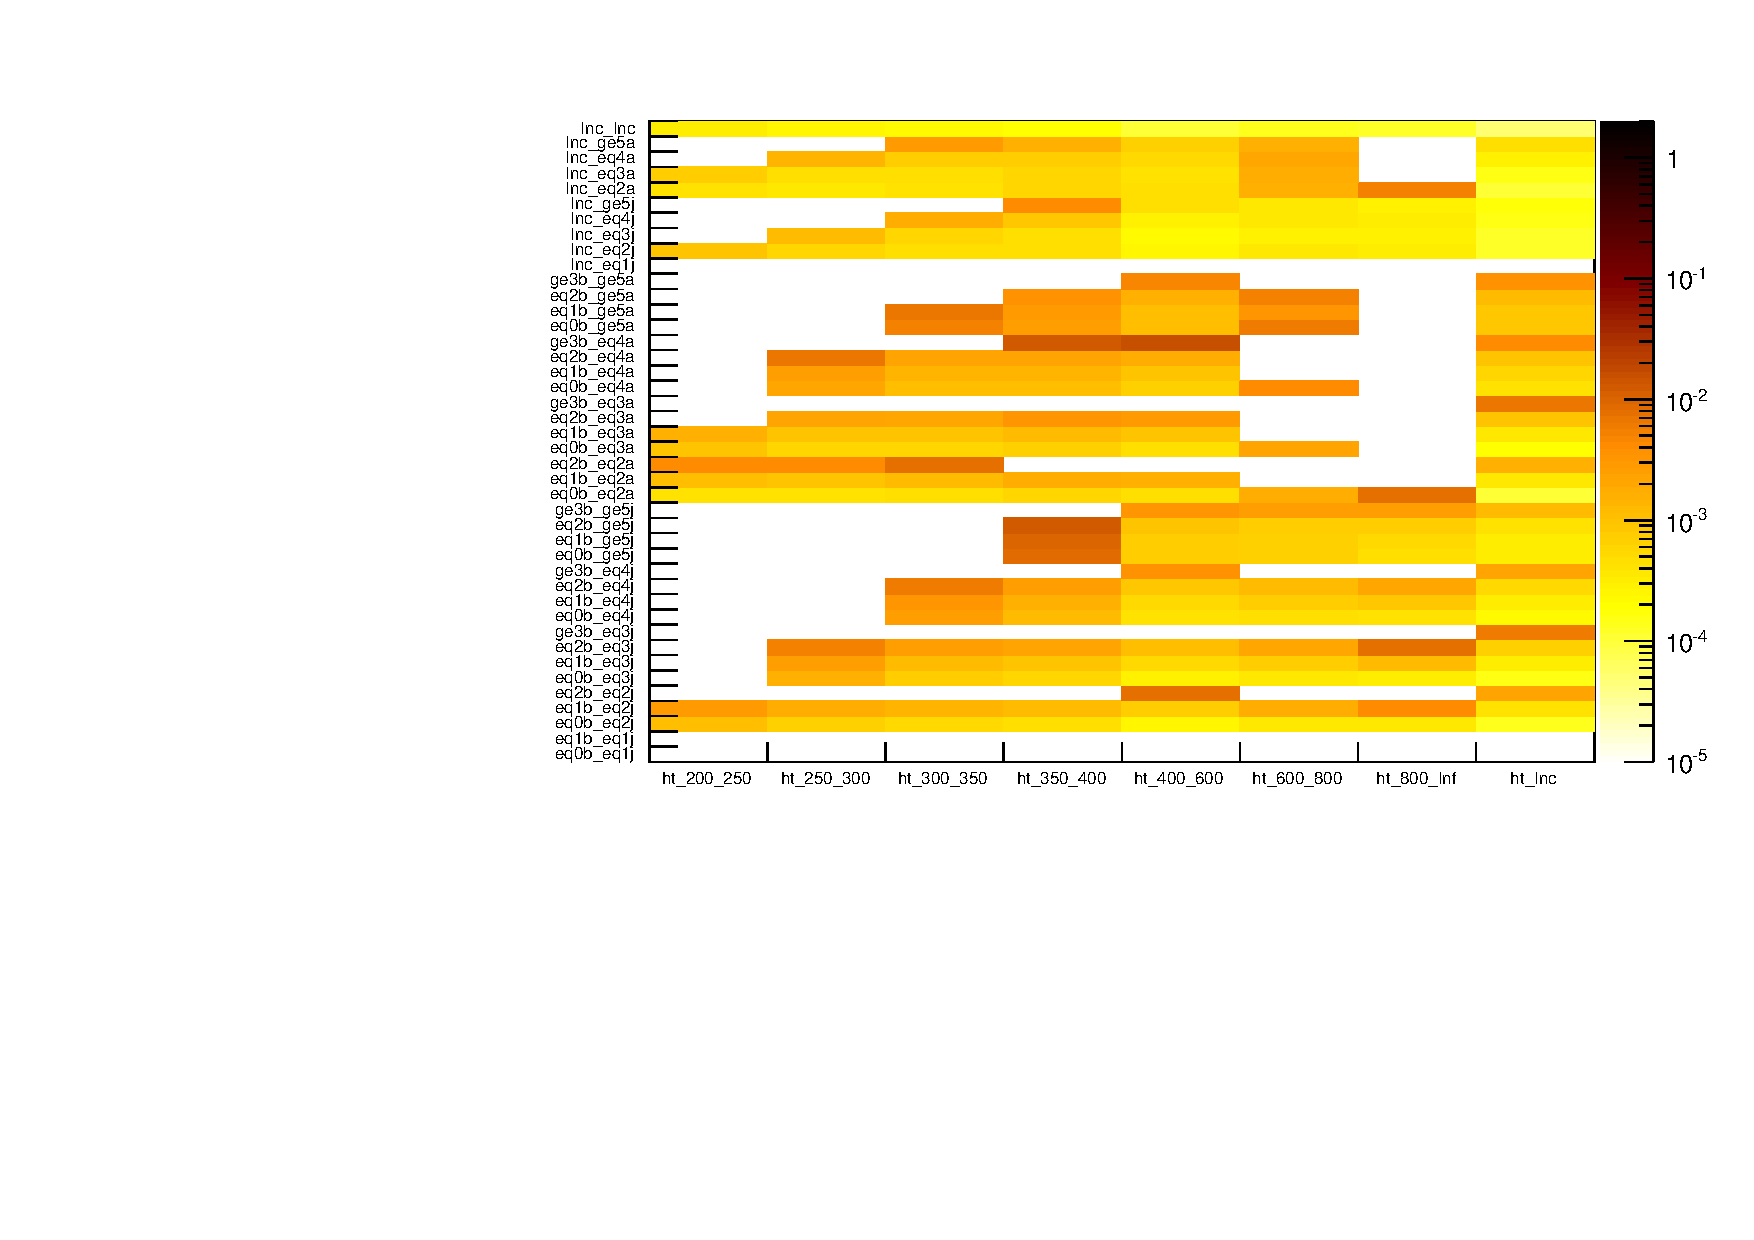
\includegraphics[width=0.5\textwidth]{figures/template/linear/frenchFlagErrComplete13_Linear2D_p1_Zinv.pdf}
  }~~
  \subfigure[\label{fig:zinv13} \zInv]{
    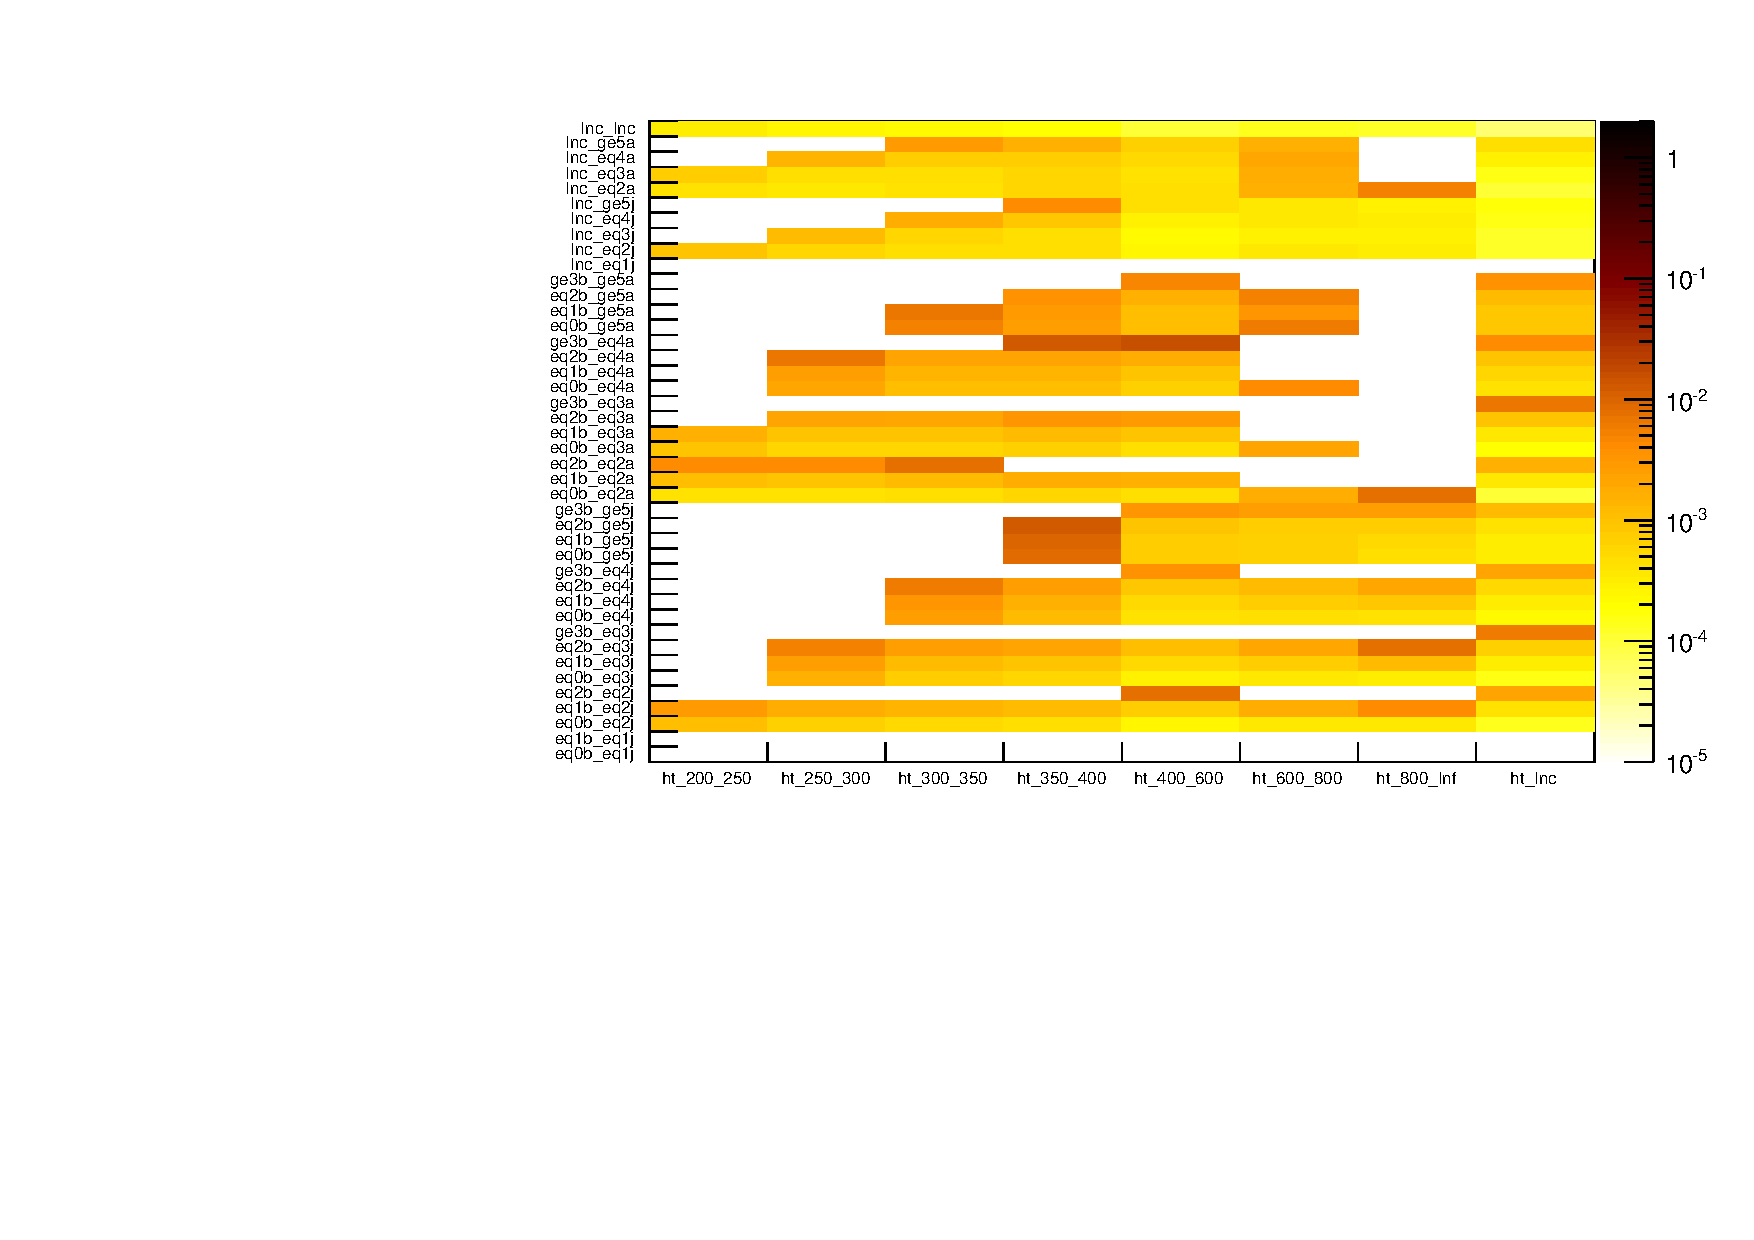
\includegraphics[width=0.5\textwidth]{figures/template/linear/frenchFlagErrComplete13_Linear2D_p1_Zinv.pdf}
  }\\
  \caption{\label{fig:expected13}
  Expected relative uncertainties on the template shown for \zInv~ in Figure~\ref{fig:zinv13} 
  and \ttbar/w in Figure~\ref{fig:ttw13} are around 1 to 10\%.}
  
\end{figure}

\begin{figure}[h!]
  \centering
  \subfigure[]{
    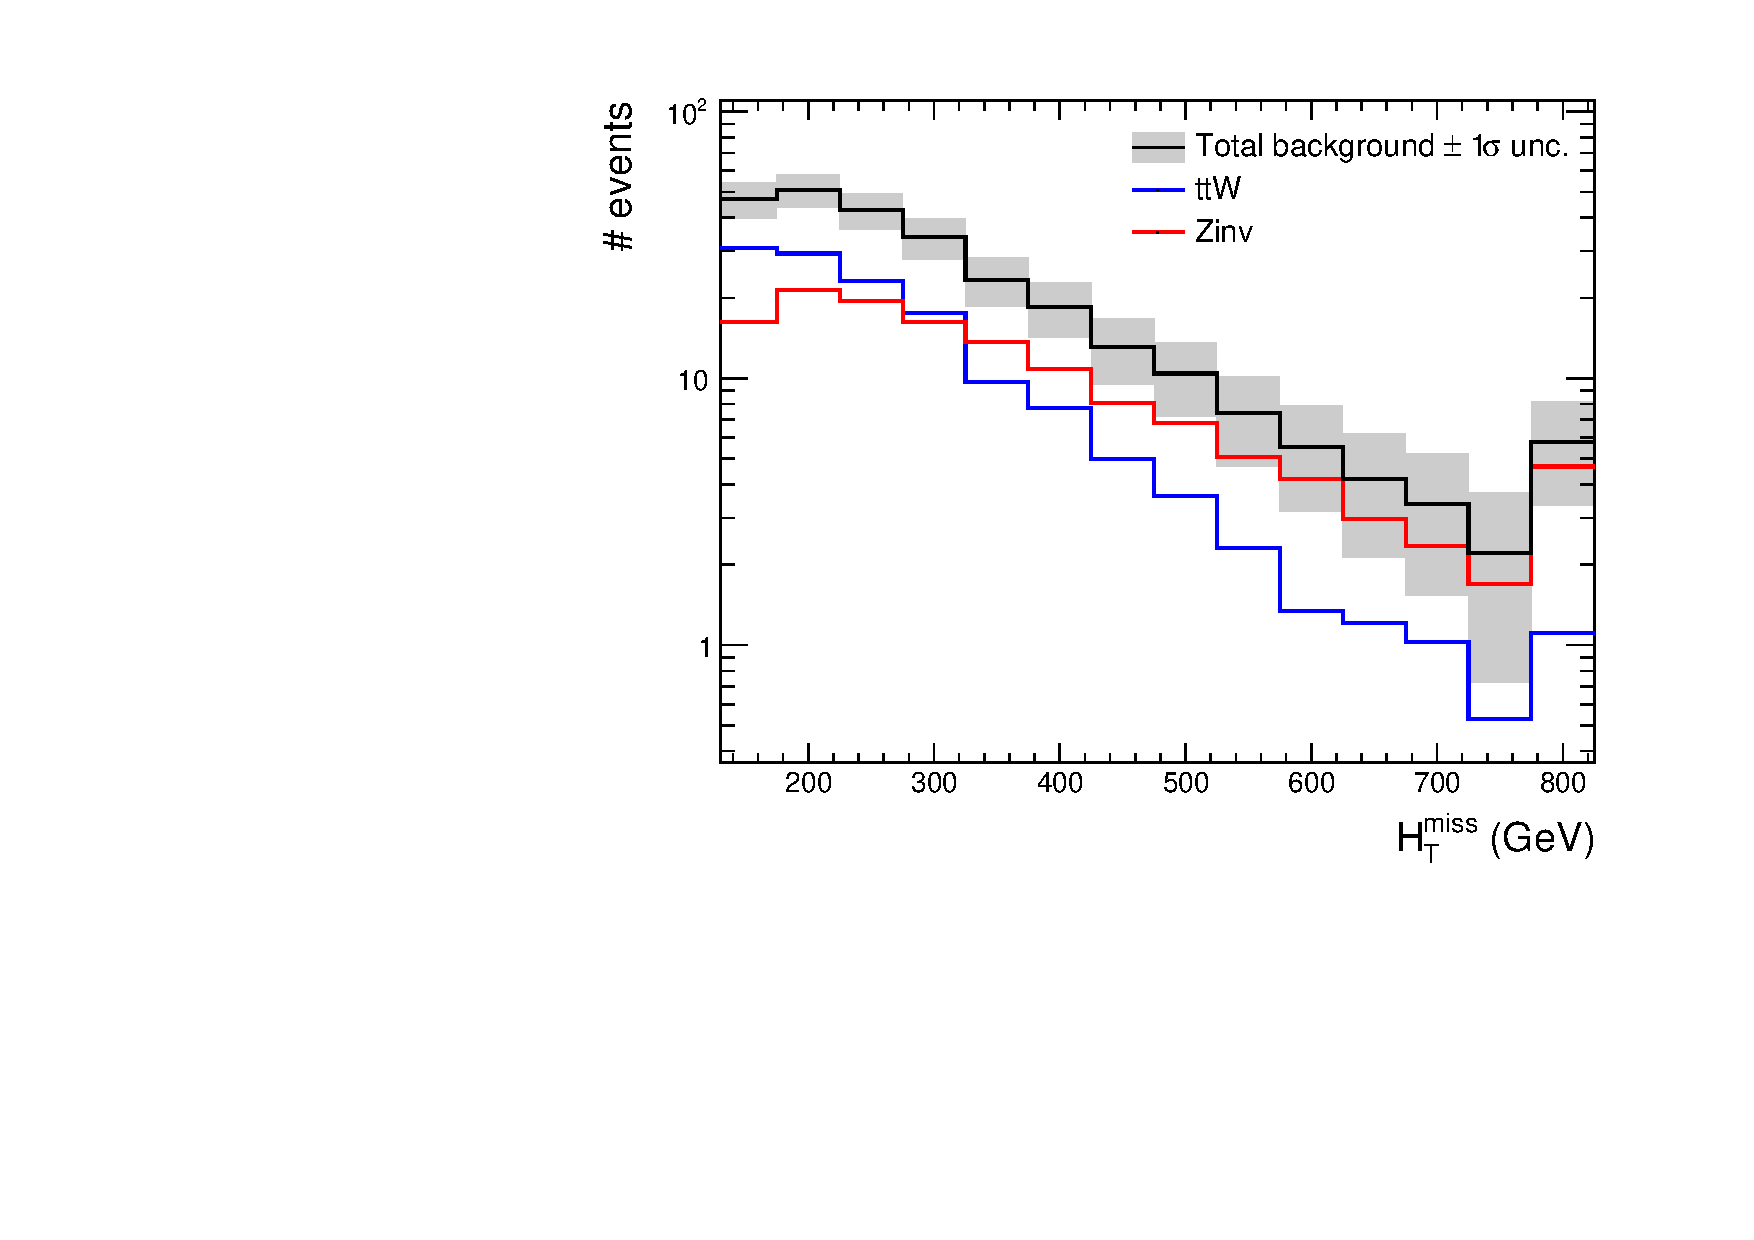
\includegraphics[width=0.5\textwidth]{figures/template/exampleTemplate13TeV.pdf}
  }\\
  \caption{\label{fig:exampleTemplate13}
  Example template for 0b,$\ge5$j and $\scalht > 800$\GeV showing the error from both
components of the background on the total background prediction.}
  
\end{figure}

\subsection{Additional uncertainties in the \mht dimension}
\label{sec:addMhtUnc}
Theoretical uncertanties due to scale differences in the data and MC agreement 
are mitigated through the procedure described in
Section~\ref{sec:mhtTemplate}. Several additional potential 
sources of uncertainty will be considered, such as
ISR, JES, PDF, b-tag scale factors, etc, as detailed below. In
general, for each source of systematic, the \mht templates are found
based on $\pm$1$\sigma$ variations in the relevant source of
uncertainty. The alternative templates reflect the magnitude of the
migration of events between bins in \mht (but not in \njet, \nb, nor
\scalht, which is encapsulated by the normalisation systematic
uncertainties from closure tests). If the systematic source is found
to be significant, the template variations will be included in the
likelihood. 

\begin{figure}[]
  \centering
  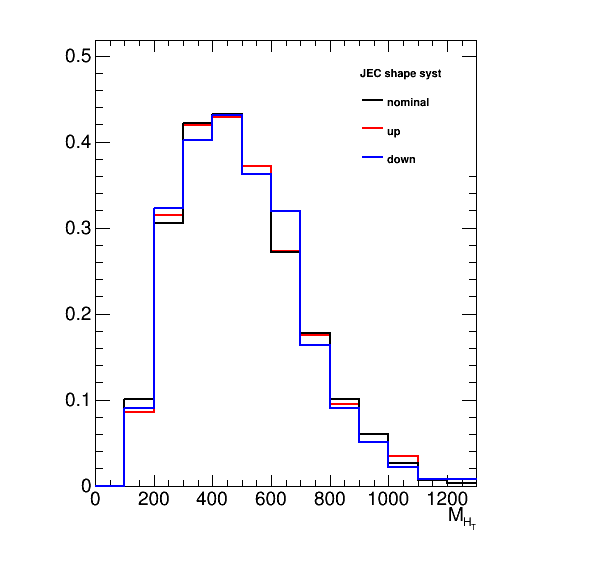
\includegraphics[width=0.5\textwidth]{figures/closureTests/mhtJetSyst_SMS_T1bbbb_2J_mGl1000_mLSP900_JEC_ge3b_ge5j_800_1600.png}
  \caption{\label{fig:jec-shape} Alternative \mht templates that
    refect uncertainties in the jet energy scale corrections for
    $\geq$5 jets, $\geq$3 b-jets, and $\scalht > 800\gev$ bin for the
    10 \ifb luminosity scenario.}
\end{figure}

An indicative behaviour is shown in Figure~\ref{fig:jec-shape} by
considering the variation of jet energy scale given the uncertainties
determined in Run~1. The relative change in the \mht distribution is
determined when varying the energy of all jets in an event up or down
according to a \pt- and $\eta$-dependent jet energy scale uncertainty
(\ie vary the event scale up and down), as recommended by the JetMET
POG. 

% \begin{figure}[]
%   \centering
%   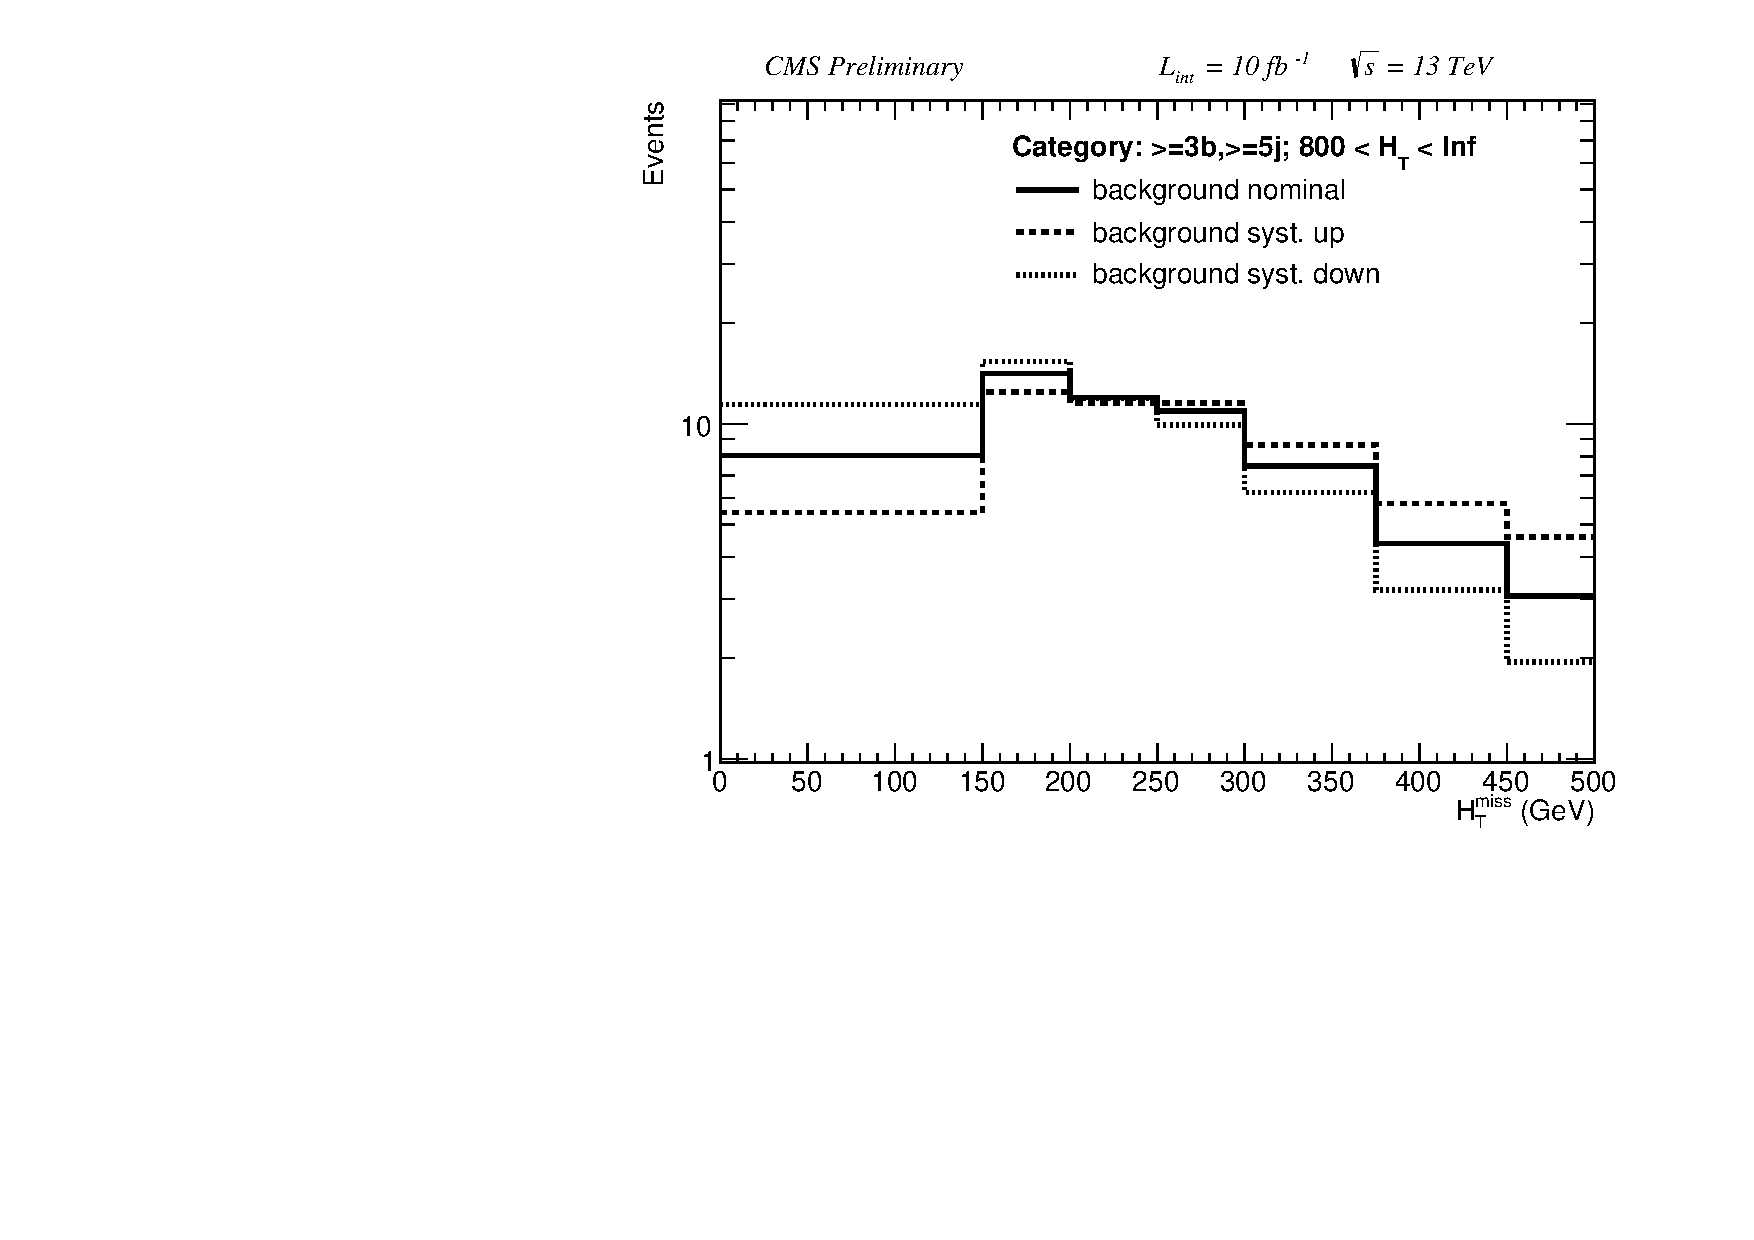
\includegraphics[width=0.7\textwidth]{figures/mhtShapeSyst/MHTShapeSyst_ge3b_ge5j_800_Inf.pdf}
%   \caption{\label{fig:mht-shape-syst-toy} 
%     The nominal \mht shape and its up/down alternative shapes for the 
%     \ttbar/W background in the $\njet \geq5$, $\nb \geq 3$
%     category for the $\HT > 800 \gev$ bin.
%   }
% \end{figure}

% %While simulation-based studies are also ongoing, some comments are
% %made below on some of the potential sources of uncertainty that are
% %expected to be dominant. This list is clearly not exhaustive.
% %
% %{\bf Jet energy scale:} 
% %
%
% %
% %{\bf PDF uncertainties:}
% %
% %\newcommand{\lcr}{Left: $\frac{\epsilon_{CTEQ6L1}}{\epsilon_{CT10}}$,
% %  center: $\frac{\epsilon_{CTEQ6L1}}{\epsilon_{MSTW08}}$, right:
% %  $\frac{\epsilon_{CTEQ6L1}}{\epsilon_{NNPDF2.1}}$}
% %
% %The samples are produced with the \verb!CTEQ6L1! PDF set by default.
% %The shape is compared with that obtained with three alternative PDF
% %sets: \verb!CT10!, \verb!NNPDF2.1!, and \verb!MSTW2008!. The envelope
% %and its uncertainties are determined following the PDF4LHC
% %recommendation~\cite{pdf4lhc}. 
% %
% %{\bf Initial state radiation:}
% %
% %Will have to cook up a recipe for this\ldots
% %
% %
% %{\bf \texorpdfstring{\mht/\met}{MHT/MET} cleaning cut:}
% %
% %The efficiencies for the requirement $\mht/\met < 1.25$ must be
% %measured in data and simulation as a function of \mht for each \scalht
% %bin. The ratio of these two efficiencies should be unity. Deviation
% %from unity is taken to represent the uncertainties on the simulation
% %modelling of this variable for processes with significant, genuine
% %\met. This can be used to define templates for the uncertainty on this
% %quantity.
% %
% %{\bf Dead ECAL filter:}
% %
% %The ratio of efficiencies observed in data and simulation for the dead
% %ECAL filter may be used as in Section~\ref{sec:sms-syst-mht-met} to
% %templates for the uncertainty from the Dead ECAL filter.
